\documentclass[11pt,a4paper,oneside]{report}

% ==================== PACKAGES ====================
\usepackage[utf8]{inputenc}
\usepackage[T1]{fontenc}
\usepackage[margin=1in]{geometry}
\usepackage{graphicx}
\usepackage{booktabs}
\usepackage{amsmath, amssymb, amsthm}
\usepackage{setspace}
\usepackage{titlesec}
\usepackage{xcolor}
\usepackage{caption}
\usepackage{float}
\usepackage{array}
\usepackage{tabularx}
\usepackage[colorlinks=true,
            linkcolor=blue!60!black,
            citecolor=blue!60!black,
            urlcolor=blue!60!black]{hyperref}

\onehalfspacing

% ==================== TITLE PAGE INFO ====================
\title{Parameter-Efficient Adaptation of SAM 2 for Sentinel-1 SAR Flood Inundation Mapping in the Indo-Gangetic Region}

\author{Aksan Gony Alif \and Mahbubur Rahman \\ Department of Computer Science and Engineering \\ BRAC University}

\date{\today}

% Shrink wide tables to text width; leave narrow tables at natural size.
\newcommand{\maxwidthtable}[1]{%
  \resizebox{\ifdim\width>\linewidth \linewidth\else \width\fi}{!}{#1}%
}

% ==================== DOCUMENT ====================
\begin{document}

% ---------- TITLE PAGE ----------
\begin{titlepage}
\centering
\vspace*{1.5cm}
{\large Computer Vision Project Thesis Report \par}
\vspace{0.5cm}
\rule{\linewidth}{0.5pt}
\vspace{0.8cm}

{\Large\bfseries Parameter-Efficient Adaptation of SAM 2 \\[0.3em] for Sentinel-1 SAR Flood Inundation Mapping in the Indo-Gangetic Region \par}

\vspace{0.5cm}
\rule{\linewidth}{0.5pt}

\vfill

{\large
\textbf{Authors} \\
Aksan Gony Alif \\[0.2em]
Mahbubur Rahman \\[0.3em]
Department of Computer Science and Engineering \\
BRAC University, Dhaka, Bangladesh \\
}

\vspace{2cm}

{\large \today}

\end{titlepage}

% ---------- ABSTRACT ----------
\chapter*{Abstract}
\addcontentsline{toc}{chapter}{Abstract}

Bangladesh sits at the confluence of the Ganges, Brahmaputra and Meghna rivers and experiences large-scale monsoon flooding almost every year, with cloud cover during the monsoon season making optical satellite imagery unreliable for emergency response. Synthetic Aperture Radar (SAR) imagery from the Sentinel-1 mission is the operational alternative because radar penetrates clouds, but its noisy single-channel intensity statistics differ fundamentally from the natural RGB images on which modern vision foundation models are pretrained. This thesis reports on the design, implementation and empirical evaluation of a parameter-efficient adaptation of the Segment Anything Model 2 (SAM 2) for Sentinel-1 SAR flood inundation mapping, with four principal contributions: a systematic empirical comparison of four parameter-efficient fine-tuning methods (Low-Rank Adaptation, Weight-Decomposed Low-Rank Adaptation, Convolutional LoRA and AdaptFormer) on two SAM-family backbones (SAM ViT-B and SAM 2 Hiera-Base-Plus) extended to three larger stretch backbones (SAM ViT-L, SAM ViT-H, SAM 2 Hiera-Large) under Conv-LoRA; a polarimetric prompt-engineering ablation that exploits the dual-polarization structure of Sentinel-1 imagery to construct three-channel pseudo-RGB inputs; a confidence-aware mechanism using Monte Carlo dropout to produce per-pixel calibrated uncertainty estimates alongside the flood maps; and a custom Pakistan-2022 SAR flood test set, built from TU Wien Sentinel-1 flood-extent labels paired with Microsoft Planetary Computer Sentinel-1 RTC imagery, providing the only true geographic-and-temporal out-of-distribution surface used in this evaluation (39 chips at Sentinel-1's native 10-metre resolution). A standalone dataset construction pipeline for the June 2022 Bangladesh-Sylhet flood event is also released alongside the codebase as future work but is not empirically evaluated here. The experimental sweep runs on a Vast.ai cloud instance with dual NVIDIA RTX PRO 5000 Blackwell GPUs, and the empirical evaluation is reported on four splits: the Sen1Floods11 hand-labeled test split (in-distribution), the Sen1Floods11 Bolivia held-out country split, a regional Pakistan subset of Sen1Floods11, and the Pakistan-2022 custom test set as the strict out-of-distribution test by both geography and time.

\vspace{1em}
\noindent\textbf{Keywords:} Segment Anything Model, parameter-efficient fine-tuning, synthetic aperture radar, flood inundation mapping, foundation models, confidence-aware learning, Bangladesh, Ganges-Brahmaputra delta.

% ---------- TABLE OF CONTENTS ----------
\tableofcontents

% ==================== CHAPTER 1: INTRODUCTION ====================
\chapter{Introduction}
\label{chap:intro}

\section{Background and Motivation}

Floods are among the most damaging natural disasters worldwide, and their economic and humanitarian costs have risen sharply over the past two decades as a consequence of climate change, accelerated urbanization in flood-prone regions, and the increasing frequency of extreme precipitation events \cite{Hu2025GlobalFloods}. Bangladesh, situated at the head of the Bay of Bengal and on the alluvial plains of the Ganges, Brahmaputra and Meghna river systems, is particularly exposed. During a typical monsoon season, between twenty and twenty-five percent of the country's land area becomes inundated, and during severe events the figure has historically reached between thirty and sixty percent. The 2022 Sylhet flash flood, which is the case study examined in this thesis, affected approximately seven point two million people across nine northeastern districts and displaced an estimated four hundred and eighty thousand people to roughly sixteen hundred institutional shelters at the peak of the event, according to United Nations Office for the Coordination of Humanitarian Affairs and International Federation of Red Cross and Red Crescent Societies reporting. Accurate, timely flood-extent mapping is therefore not a purely scientific question but an operational humanitarian requirement that informs evacuation, relief logistics, agricultural recovery and infrastructure repair.

The dominant remote sensing modality for global flood monitoring is the Sentinel-1 mission of the European Space Agency, which provides free and open Synthetic Aperture Radar imagery at ten-meter resolution with a six-day revisit time over most of the world. The reason Sentinel-1 dominates over optical alternatives such as Sentinel-2 and Landsat is straightforward and physical, namely that radar wavelengths penetrate clouds. During the South Asian monsoon, cloud cover over Bangladesh routinely exceeds eighty percent for weeks at a time, which renders optical imagery essentially useless precisely when flood mapping is most urgent. SAR observations remain available regardless of weather conditions, day or night.

The technical challenge is that SAR imagery is fundamentally different from the natural RGB photographs on which contemporary computer vision models are trained. SAR is an active sensing modality that records the backscattered intensity of a transmitted microwave pulse, and its statistics are dominated by multiplicative speckle noise rather than the additive Gaussian noise that characterizes optical imaging. SAR images are typically single-channel or dual-channel, with the two channels in Sentinel-1 corresponding to vertically polarized transmit with vertically polarized receive (VV) and vertically polarized transmit with horizontally polarized receive (VH). The dynamic range of SAR data is logarithmic, expressed in decibels, and visual interpretation requires understanding that water bodies appear dark because their smooth surfaces specularly reflect the radar pulse away from the satellite, whereas vegetation and buildings appear bright because their geometrically complex surfaces produce strong volumetric and double-bounce backscatter. None of these characteristics are present in the natural RGB images on which large vision foundation models are trained.

The recent emergence of foundation models in computer vision, most prominently the Segment Anything Model released by Meta in 2023 \cite{Kirillov2023SAM} and its successor SAM 2 in 2024 \cite{Ravi2025SAM2}, raises a natural question for the remote sensing community: can these models be adapted to work well on SAR data, and if so, what is the right adaptation strategy given limited computational budgets? The naive approach of full fine-tuning is impractical because the smallest publicly released SAM variant has approximately ninety-one million parameters and the largest exceeds six hundred million, and fine-tuning a model of this size requires multiple high-end GPUs. The alternative is parameter-efficient fine-tuning, a family of techniques originally developed for adapting large language models, which freezes the bulk of the pretrained weights and trains only a small number of additional parameters, typically below five percent of the model. Parameter-efficient fine-tuning techniques such as Low-Rank Adaptation \cite{Hu2022LoRA}, Weight-Decomposed Low-Rank Adaptation \cite{Liu2024DoRA}, Convolutional LoRA \cite{Zhong2024ConvLoRA} and AdaptFormer \cite{Chen2022AdaptFormer} have been demonstrated to match or approach full fine-tuning performance at a small fraction of the compute and storage cost.

A second motivating context is the rise of foundation models specifically built for remote sensing imagery, including SkySense \cite{Guo2024SkySense}, Prithvi developed by IBM and NASA, and TerraMind developed by IBM and the European Space Agency. While these models reduce the modality gap by pretraining on satellite data including Sentinel-1, they typically demand substantial compute for fine-tuning and are not optimized for the specific task of flood inundation mapping. There is therefore a methodological niche for work that adapts the more accessible SAM family of models to SAR specifically, with carefully chosen parameter-efficient mechanisms and domain-aware prompt engineering.

\section{Problem Statement}

Despite the operational importance of SAR-based flood mapping and the rapid progress in vision foundation models, the intersection of these two areas remains underexplored at peer-reviewed venues. A recent and thorough survey of the literature reveals a specific gap. The Segment Anything Model has been adapted to SAR for landcover classification by ClassWise-SAM-Adapter \cite{Pu2025CWSAM}, but not for flood inundation mapping. SAM has been adapted to remote sensing imagery in general by a number of works, but most of these target optical imagery and do not address the distinctive statistics of SAR. SAM 2, the successor model released in 2024, has been applied to remote sensing tasks such as oil-spill segmentation and optical change detection, but its application to SAR flood mapping has not yet appeared in peer-reviewed Q1 journals or A-rank conference proceedings. Furthermore, no published work combines SAM-family adaptation with a confidence-aware mechanism that produces calibrated uncertainty estimates alongside flood maps, despite the fact that operational flood response decisions are precisely the kind of high-stakes application where uncertainty information is most valuable.

This thesis addresses this gap by proposing, implementing and evaluating a parameter-efficient adaptation of SAM 2 for Sentinel-1 SAR flood inundation mapping, augmented with a confidence-aware mechanism inspired by recent work on confidence-aware retrieval-augmented systems, and validated on a custom Pakistan-2022 test set built from the August-September 2022 Indo-Gangetic monsoon flood event (the same meteorological system that produces Bangladesh's annual flooding).

\section{Research Questions}

The thesis is organized around four research questions, each of which corresponds to one chapter of the experimental program.

The first research question asks which parameter-efficient fine-tuning method is most effective for adapting SAM and SAM 2 to Sentinel-1 SAR flood inundation mapping. Specifically, the comparison includes Low-Rank Adaptation, Weight-Decomposed Low-Rank Adaptation, Convolutional LoRA, and AdaptFormer-style adapters, evaluated across two backbone scales corresponding to SAM ViT-B and SAM 2 Hiera-Base-Plus. The hypothesis is that methods which inject local convolutional inductive biases, such as Convolutional LoRA, will outperform pure low-rank linear adaptations on SAR because the local statistics of speckle and water boundaries reward locality-aware feature extraction.

The second research question asks whether systematic polarimetric prompt engineering improves SAM-family performance on Sentinel-1 imagery. SAM was pretrained to consume three-channel RGB inputs, so when adapting it to dual-polarization Sentinel-1 data the practitioner must construct a three-channel pseudo-image from the available VV and VH backscatter coefficients. The prevailing convention, used informally across industry tutorials, is to stack VV, VH and the ratio of VV to VH, but this choice has not been systematically ablated against alternatives such as VV-VH difference, replicated single-channel inputs or learned channel composition.

The third research question, and the one most directly aligned with the broader research interests of the author, asks whether a confidence-aware mechanism can be incorporated into the adapted SAM 2 model to produce calibrated uncertainty estimates without sacrificing segmentation accuracy. The proposed mechanism draws on Monte Carlo dropout and deep ensembling and is structured to mirror the confidence-weighted memory entries used in Confidence-Aware Episodic Memory architectures for retrieval-augmented language models.

The fourth research question is empirical and regional, asking how well a model trained on the global Sen1Floods11 benchmark generalizes to a specific Indo-Gangetic monsoon flood event that is held out by both geography and time. The Indo-Gangetic floodplain has physiographic features, including large tracts of flooded vegetation, dense rural settlements and complex river channel networks, that are partially represented in Sen1Floods11 but whose 2022 monsoon-season acquisitions are entirely out-of-distribution. The thesis constructs a custom Pakistan-2022 test set covering the August-September 2022 Indo-Gangetic monsoon flood event, derived from the TU Wien Sentinel-1 flood-extent label release paired with matching Microsoft Planetary Computer Sentinel-1 RTC imagery, and uses this set to characterize the out-of-distribution generalization of the trained models. A separate construction pipeline targeting the June 2022 Bangladesh-Sylhet flood event is shipped as a future-work artifact in this thesis but its chips are not empirically evaluated here.

\section{Contributions}

The thesis makes four primary contributions. The first is a systematic empirical comparison of four parameter-efficient fine-tuning methods applied to the SAM and SAM 2 backbones for the specific task of Sentinel-1 SAR flood inundation mapping, with full ablations across three random seeds and reproducibility through publicly released code. The second is a polarimetric prompt-engineering ablation that establishes a defensible convention for constructing three-channel pseudo-RGB inputs from dual-polarization SAR data and that localizes a striking out-of-distribution failure mode to the cross-polarization channel. The third is the first application of a confidence-aware mechanism, ported from confidence-aware retrieval-augmented systems, to SAR flood mapping with SAM 2, accompanied by both aggregate calibration analysis (expected calibration error, reliability diagrams) and a pointwise selective-prediction analysis that surfaces a substantive negative finding about MC-dropout uncertainty on out-of-distribution events. The fourth is the construction and public release of a Pakistan-2022 SAR flood test set ($39$ chips at Sentinel-1's native 10-metre resolution, built from TU Wien Sentinel-1 flood-extent labels paired with Microsoft Planetary Computer Sentinel-1 RTC imagery via a documented acquisition pipeline), providing the only SAM-evaluation surface in the public literature that combines temporal and geographic out-of-distribution shift on Sentinel-1. A separate Bangladesh-2022-Sylhet dataset construction pipeline is also released as future work but its chips are not empirically evaluated in this thesis.

\section{Thesis Organization}

The remainder of this report is organized as follows. Chapter \ref{chap:litreview} surveys the literature on vision foundation models and their adaptation, on SAR flood mapping with deep learning, and on remote sensing foundation models, and articulates the specific research gap that this thesis addresses. Chapter \ref{chap:methodology} describes the proposed methodology in detail, including the choice of backbone, the parameter-efficient fine-tuning methods to be compared, the polarimetric prompt-engineering protocol, the confidence-aware mechanism, and the dataset construction strategy. Chapter \ref{chap:experimental} specifies the experimental setup, including hardware, software stack, training protocol and hyperparameter choices. Chapter \ref{chap:results} presents the empirical results across all four evaluation splits, the polarimetric ablation, the confidence calibration analysis, and the OOD-gap and ensemble analyses. Chapter \ref{chap:conclusion} concludes the proposal and outlines directions for future extension.

% ==================== CHAPTER 2: LITERATURE REVIEW ====================
\chapter{Literature Review}
\label{chap:litreview}

\section{Vision Foundation Models and the Segment Anything Family}

The Segment Anything Model, introduced by Kirillov and colleagues at Meta AI Research and presented at the International Conference on Computer Vision in 2023 \cite{Kirillov2023SAM}, marked a turning point in segmentation research by demonstrating that a single promptable model trained on a sufficiently large and diverse dataset could perform competitive zero-shot segmentation across a wide range of downstream tasks. The model architecture comprises three components, namely a Vision Transformer image encoder that produces a dense feature representation of the input image, a prompt encoder that converts user-supplied prompts such as points, boxes or coarse masks into embedding vectors, and a lightweight mask decoder that fuses the image features and prompt embeddings to produce a segmentation mask. The training corpus, called SA-1B, contains over one billion masks across eleven million images and was constructed through a partly model-assisted data engine. The result is a model whose released ViT-Huge variant exhibits remarkably strong zero-shot generalization on natural RGB images.

The successor model, Segment Anything Model 2, was released in 2024 and presented at the International Conference on Learning Representations in 2025 \cite{Ravi2025SAM2}, where it received an Oral presentation. SAM 2 introduces three significant changes relative to its predecessor. First, it replaces the plain Vision Transformer encoder with a Hiera architecture that produces multi-scale features more naturally suited to dense prediction. Second, it adds a streaming memory module that allows the model to propagate segmentations across video frames, although this same module can be repurposed for paired-image tasks such as bi-temporal change detection. Third, the released models span a range of sizes from Hiera-Tiny at approximately thirty-nine million parameters through Hiera-Small at forty-six million and Hiera-Base-Plus at approximately eighty-one million to Hiera-Large at approximately two hundred and twenty-four million, and the smaller variants are noticeably faster than the corresponding SAM variants while achieving better mask quality.

A substantial follow-up literature has explored the limitations of SAM and proposed targeted improvements. HQ-SAM \cite{Ke2023HQSAM} introduces a learnable High-Quality Output Token in the mask decoder, fused with early and final ViT features, and trains it on a curated dataset of forty-four thousand high-quality masks. The result is a model that produces visibly cleaner mask boundaries on objects with thin or intricate structures, while preserving the zero-shot capabilities of the original SAM. Stable-SAM addresses the observation that SAM's automatic prompt generation is unstable in noisy or low-contrast images by introducing a stability-promoting training objective. EfficientSAM uses masked-image pretraining and distillation to produce a smaller, faster SAM variant with negligible accuracy degradation.

Most relevant to the present thesis is the work on adapting SAM to medical imaging. MedSAM, published in Nature Communications in 2024 \cite{Ma2024MedSAM} and now cited several thousand times, full-fine-tunes SAM on a curated corpus of over one and a half million medical mask annotations spanning radiology, microscopy and pathology. MedSAM is the most prominent published example of adapting a general-purpose foundation model to a non-RGB modality and serves as a template for the kind of writeup that the present thesis aims to produce, although the methodology differs substantially because the present work uses parameter-efficient fine-tuning rather than full fine-tuning.

\section{Parameter-Efficient Fine-Tuning}

Parameter-efficient fine-tuning, often abbreviated PEFT, is a family of techniques originally developed in the language modeling community to enable adaptation of very large pretrained models without the computational cost of updating all parameters. The defining principle is to freeze the pretrained weights and to introduce a small number of additional trainable parameters, typically below five percent of the model, which absorb the task-specific signal during fine-tuning.

Low-Rank Adaptation, introduced by Hu and colleagues at the International Conference on Learning Representations in 2022 \cite{Hu2022LoRA}, is the most widely adopted PEFT method. The core idea is that the weight update induced by fine-tuning, denoted $\Delta W$, can be approximated by a low-rank decomposition $\Delta W = BA$ where $B$ and $A$ are matrices of dimensions $d \times r$ and $r \times d$ respectively, with $r$ much smaller than $d$. The pretrained weight matrix $W$ is frozen, and only $A$ and $B$ are trained, which reduces the number of trainable parameters by orders of magnitude. LoRA is now standard practice and is implemented in widely used libraries such as the HuggingFace PEFT package.

Weight-Decomposed Low-Rank Adaptation, presented as an Oral paper at the International Conference on Machine Learning in 2024 \cite{Liu2024DoRA}, refines LoRA by decomposing the pretrained weight matrix into a magnitude vector and a directional matrix, and applies LoRA-style updates only to the directional component. This decomposition is motivated by analyses showing that fine-tuning predominantly modifies the direction rather than the magnitude of weights, and DoRA closes a substantial portion of the gap between LoRA and full fine-tuning at essentially the same parameter cost.

Convolutional LoRA, presented at the International Conference on Learning Representations in 2024 \cite{Zhong2024ConvLoRA}, was developed specifically for adapting SAM to specialized visual domains including medical imaging and remote sensing. The method augments LoRA with ultra-lightweight convolutional parameters that inject locality-aware inductive bias into the plain ViT encoder, addressing a known weakness of pure linear low-rank adaptations on dense visual prediction tasks. The empirical results in the original paper show consistent improvements over plain LoRA across multiple specialized domains, which makes Convolutional LoRA a natural candidate for SAR adaptation where local speckle statistics are central.

Visual Prompt Tuning, presented at the European Conference on Computer Vision in 2022 \cite{Jia2022VPT}, takes a different approach by prepending a small number of learnable prompt tokens to the input sequence of a frozen Vision Transformer. AdaptFormer, presented at the Conference on Neural Information Processing Systems in 2022 \cite{Chen2022AdaptFormer}, inserts parallel adapter modules into the feed-forward block of each transformer layer. Both methods provide alternative inductive biases relative to LoRA and are included in the comparison plan of the present thesis.

\section{SAM Adaptation for Remote Sensing}

A growing body of work has explored the adaptation of SAM to remote sensing imagery. RingMo-SAM, published in IEEE Transactions on Geoscience and Remote Sensing in 2023 \cite{Yan2023RingMoSAM}, builds a SAM-based foundation model that handles both optical and SAR remote sensing data, with a category-decoupling mask decoder for instance-aware segmentation. RSPrompter, also published in IEEE Transactions on Geoscience and Remote Sensing in 2024 \cite{Chen2024RSPrompter}, proposes to learn the generation of appropriate prompts for SAM in remote sensing, removing the requirement for manual prompt input and enabling automated instance segmentation across diverse datasets including SAR ship detection.

ClassWise-SAM-Adapter, accepted in IEEE Journal of Selected Topics in Applied Earth Observations and Remote Sensing in 2025 \cite{Pu2025CWSAM}, is the closest existing work to the present thesis. The authors freeze most of SAM's parameters, insert lightweight adapters into the encoder, and add a class-aware mask decoder for multi-class semantic segmentation of Sentinel-1 SAR images. The application target is landcover classification rather than flood inundation mapping, which leaves the latter an open problem, but the methodological similarity is sufficient that ClassWise-SAM-Adapter is the natural baseline against which the present thesis must compare.

A separate strand of work has developed remote-sensing-specific foundation models. SkySense, presented at the Conference on Computer Vision and Pattern Recognition in 2024 \cite{Guo2024SkySense}, is a 2.06-billion parameter model pretrained on a curated multimodal dataset of twenty-one and a half million temporal sequences spanning high-resolution optical, multispectral Sentinel-2 and SAR Sentinel-1 modalities, using a multi-granularity contrastive learning objective. SkySense is the most relevant remote sensing foundation model for SAR-aware applications, and its public release of pretrained weights makes it a viable alternative backbone, although its compute requirements for fine-tuning are significantly higher than SAM ViT-B. The Prithvi family of models, developed jointly by IBM and NASA, has been demonstrated for flood inundation mapping on Sen1Floods11 with strong out-of-distribution generalization, and has been further refined in the Prithvi-EO 2.0 release. TerraMind, developed by IBM in collaboration with the European Space Agency, is a multimodal generative model for Earth observation that includes SAR among its supported modalities.

The PANGAEA benchmark \cite{Marsocci2024PANGAEA} provides a head-to-head comparison of geospatial foundation models against simple convolutional baselines such as U-Net on a panel of remote sensing tasks including Sen1Floods11. A central and somewhat sobering finding of PANGAEA is that a vanilla U-Net of approximately thirty million parameters often matches or exceeds large foundation models on Sen1Floods11 across all training-data fractions, with the U-Net reaching a mean Intersection-over-Union of roughly ninety-one percent on the Sentinel-2 split. This finding does not invalidate the foundation model paradigm, but it does mean that any foundation-model-based work on Sen1Floods11 must include and honestly report a U-Net baseline, and must be prepared to articulate what the foundation model adds beyond what U-Net already provides. The present thesis takes this requirement seriously and includes U-Net as a primary baseline.

\section{SAR Flood Mapping with Deep Learning}

Sen1Floods11, introduced by Bonafilia and colleagues at the CVPR 2020 workshops \cite{Bonafilia2020Sen1Floods11}, is the canonical benchmark dataset for Sentinel-1 SAR flood mapping. It comprises four hundred and forty-six hand-labeled five-hundred-and-twelve-by-five-hundred-and-twelve pixel chips drawn from eleven flood events distributed across the globe, supplemented by four thousand three hundred and eighty-five weakly labeled chips per sensor for warmup training, where the weak labels are released independently for the Sentinel-1 and Sentinel-2 modalities covering the same scenes. The dataset has become the standard benchmark for SAR flood mapping research and is used by virtually every paper in the area.

DAM-Net, published in the ISPRS Journal of Photogrammetry and Remote Sensing in 2024 \cite{Saleh2024DAMNet}, represents the current state of the art in transformer-based SAR flood detection. The architecture uses a Siamese Vision Transformer backbone to process pre-flood and post-flood SAR pairs, augmented with a temporal differential fusion module that integrates change features and high-level semantic tokens. DAM-Net achieves an F1 score above ninety-six percent and an Intersection-over-Union above ninety-three percent on the S1GFloods benchmark, which the same authors release alongside the paper. DAM-Net is the strongest non-foundation-model transformer baseline in the area and serves as the principal SOTA reference point for the present thesis.

DeepSARFlood \cite{Sharma2025DeepSARFlood}, published in Science of Remote Sensing in 2025, takes a different approach by using a deep ensemble of Vision Transformer and CNN-Vision-Transformer hybrid models, achieving an Intersection-over-Union of 0.72 on Sen1Floods11. The method explicitly produces uncertainty estimates through ensemble disagreement, which is the closest published analog to the confidence-aware mechanism proposed in this thesis. DeepSARFlood is demonstrated on the 2022 Pakistan flood and the 2020 Assam flood, both of which are deltaic monsoon events similar to the Bangladesh case study.

LiST-Net, also published in IEEE Transactions on Geoscience and Remote Sensing in 2024, proposes a lightweight SAR transformer network with dimension-wise interactive attention. The Hu and colleagues paper in Nature Communications in 2025 \cite{Hu2025GlobalFloods} presents a global multi-temporal flood mapping product based on ten years of Sentinel-1 data, providing operational context for the academic methods discussed above.

\section{Bangladesh-Specific Flood Mapping}

{\sloppy A focused literature exists on flood mapping for Bangladesh and the broader Ganges-Brahmaputra delta, but it has not yet incorporated transformer-based or foundation-model-based methods. Uddin and colleagues, in Remote Sensing in 2019, present an operational flood mapping pipeline for Bangladesh using multi-temporal Sentinel-1 imagery and threshold-based water detection, focusing on the 2017 monsoon flood. Singha and colleagues, in the ISPRS Journal of Photogrammetry and Remote Sensing in 2020, identify floods and flood-affected paddy rice fields in Bangladesh using Sentinel-1 imagery and Google Earth Engine. Lemenkova in Water in 2024 \cite{Lemenkova2024Ganges} presents a deep learning-based monitoring of flood dynamics in the Ganges Delta, using convolutional architectures rather than foundation models. Roth and colleagues, in Natural Hazards and Earth System Sciences in 2023 \cite{Roth2023Pakistan}, use Sentinel-1 to analyze the severe 2022 Pakistan flood with a Bayesian approach.\par}

To the best of the present author's knowledge, no published work combines the Segment Anything Model family with Sentinel-1 SAR for flood inundation mapping in Bangladesh, and no Bangladesh-specific test set for SAR flood mapping has been publicly released alongside a parameter-efficient fine-tuning study. This regional gap is one of the principal motivating gaps for the present thesis.

\section{Research Gap}

The literature review reveals four converging gaps that together justify the proposed research. First, while SAM has been adapted to remote sensing imagery in general and to SAR landcover classification specifically through ClassWise-SAM-Adapter, no peer-reviewed Q1 or A-rank work has applied SAM-family models to Sentinel-1 SAR flood inundation mapping. Second, SAM 2, which offers a stronger encoder, multi-scale features and a memory module that is naturally suited to bi-temporal change detection, has not yet been applied to SAR flood mapping in any published work. Third, no published work combines SAM-family adaptation with a confidence-aware mechanism that produces calibrated uncertainty estimates for SAR flood maps, despite the operational importance of uncertainty in flood-response decisions. Fourth, no released SAM-evaluation surface combines temporal and geographic out-of-distribution shift on a public reproducible Sentinel-1 acquisition, leaving the regional-generalization question for Indo-Gangetic monsoon flooding unanswered.

The present thesis addresses the first three gaps directly with empirical results, addresses the fourth gap by constructing and releasing the Pakistan-2022 OOD test set, and ships a Bangladesh-2022-Sylhet construction pipeline as a future-work artifact toward extending the regional coverage of the fourth gap.

% ==================== CHAPTER 3: METHODOLOGY ====================
\chapter{Methodology}
\label{chap:methodology}

\section{Overall Framework}

The proposed framework adapts SAM 2 to Sentinel-1 SAR flood inundation mapping through a four-stage pipeline. The first stage is data preparation, in which dual-polarization Sentinel-1 imagery is converted into three-channel pseudo-RGB inputs using a chosen polarimetric composition, then tiled and normalized for training (no training-time augmentation is applied). The second stage is parameter-efficient adaptation, in which the bulk of SAM 2's pretrained weights are frozen and a small set of trainable parameters is introduced according to one of four PEFT methods. The third stage is the confidence-aware mechanism, which augments the trained model with a procedure for producing calibrated per-pixel uncertainty estimates alongside flood-extent predictions. The fourth stage is evaluation, which compares the trained models on the Sen1Floods11 in-distribution test split, the Sen1Floods11 Bolivia held-out country split, a regional Pakistan subset of Sen1Floods11, and the custom Pakistan-2022 Indo-Gangetic-monsoon test set built in this work as the strict geographic-and-temporal out-of-distribution evaluation.

\section{Backbone Selection}

The thesis evaluates two principal backbone variants and three stretch backbones. The principal variants are SAM ViT-B (the canonical baseline used by nearly every SAM adaptation paper in the literature, approximately ninety-one million parameters) and SAM 2 Hiera-Base-Plus (the primary novel-contribution backbone, approximately eighty-one million parameters, with multi-scale feature outputs through the Hiera architecture and the streaming memory module that the confidence-aware mechanism can exploit). The stretch backbones are SAM ViT-L (three hundred and eight million parameters), SAM ViT-H (six hundred and thirty-six million parameters) and SAM 2 Hiera-Large (two hundred and twenty-four million parameters). All five backbones are evaluated under Conv-LoRA at three random seeds in the experimental sweep described in Chapter \ref{chap:results}; the four principal PEFT methods (LoRA, DoRA, Conv-LoRA, AdaptFormer) are evaluated at three seeds each only on the two principal backbones, since the four-by-five-by-three matrix of PEFT-by-backbone-by-seed would exceed the time budget without changing the principal conclusion. The stretch backbones serve to test whether the PEFT findings on the small backbones extrapolate cleanly to larger model sizes; that question is answered in Section \ref{sec:results-stretch}.

\section{Parameter-Efficient Fine-Tuning Methods}

Four parameter-efficient fine-tuning methods are evaluated under a common training protocol. The first is plain Low-Rank Adaptation, applied to the fused query-key-value projection and the attention output projection of every transformer block in the image encoder, with rank set to eight as a starting point and ablated over the values four, eight and sixteen. The second is Weight-Decomposed Low-Rank Adaptation, applied to the same projection matrices with the same rank schedule, which separates the magnitude and direction of weight updates and trains only the directional component with low-rank approximation. The third is Convolutional LoRA, which augments the LoRA decomposition with ultra-lightweight convolutional layers that introduce locality-aware inductive bias into the otherwise plain Vision Transformer encoder. The fourth is AdaptFormer, which inserts parallel feed-forward adapter modules into each transformer block and is implemented manually following the reference code released alongside the original paper.

For all four methods, the prompt encoder is frozen entirely, and the mask decoder is either fully fine-tuned at low learning rate or augmented with LoRA-rank-four adapters. The choice between full mask-decoder fine-tuning and LoRA-augmented mask-decoder fine-tuning is itself a small ablation that is reported alongside the main comparison.

\section{Polarimetric Prompt Engineering}

Sentinel-1 imagery is dual-polarization, providing VV and VH backscatter coefficients at each pixel. The Segment Anything Model and its successor were both pretrained on three-channel RGB inputs, so the practitioner must construct a three-channel pseudo-RGB image from the available SAR data. Three candidate compositions are evaluated. The first composition stacks VV in the first channel, VH in the second channel and the ratio of VV to VH in the third channel, where the ratio is computed in linear power and then converted to decibels. This composition is the prevailing convention in industry tutorials. The second composition stacks VV in the first channel, VH in the second channel and the difference between VV and VH, computed in decibels, in the third channel, which has a more direct physical interpretation as a measure of polarization contrast. The third composition replicates VV across all three channels, ignoring VH entirely, which serves as a single-polarization control. All compositions are followed by percentile clipping at the second and ninety-eighth percentiles to suppress speckle outliers, and by per-channel mean and standard-deviation normalization computed once on the Sen1Floods11 training split and held fixed thereafter.

\section{Confidence-Aware Mechanism}

The confidence-aware mechanism is the principal methodological contribution that distinguishes this thesis from prior work. The proposed implementation has two variants, of which one will be selected based on time and resource constraints. The first variant is Monte Carlo dropout applied to the mask decoder of the trained model. At inference time, dropout layers in the decoder remain active, and twenty independent forward passes are run for each input chip. The mean of the resulting probability maps serves as the final flood-extent prediction, and the per-pixel standard deviation across passes serves as the uncertainty estimate. The second variant is a deep ensemble of five independently trained LoRA seeds, each with a different random initialization, and aggregates the predictions through mean and standard deviation in the same way. Deep ensembles generally provide better-calibrated uncertainty than Monte Carlo dropout but multiply training cost by a factor of five.

A more ambitious extension, which is implemented if time permits, is a confidence-weighted memory bank for SAM 2. In SAM 2's original design, the memory module stores feature representations of previously processed video frames and uses them via cross-attention when processing the current frame. For bi-temporal SAR flood mapping, the pre-flood image plays the role of the previously processed frame and the post-flood image plays the role of the current frame. The proposed extension augments the memory entries with confidence scores derived from the model's own probability estimates, and modifies the cross-attention operation to weight memory entries by these confidence scores. The intent is to mirror the confidence-weighted memory entries used in Confidence-Aware Episodic Memory architectures for retrieval-augmented language models, where higher-confidence stored entries exert proportionally stronger influence on retrieval-conditioned generation.

Calibration is evaluated using the expected calibration error metric and visualized through reliability diagrams. The expected calibration error partitions the probability range into bins, computes the difference between the average predicted probability and the empirical accuracy within each bin, and reports the weighted mean of these differences across bins. A well-calibrated model has expected calibration error close to zero and a reliability diagram that lies on the diagonal.

\section{Datasets}

The experimental pipeline draws on three publicly distributed datasets. The first provides the in-distribution training and evaluation data, and the second and third provide out-of-distribution generalization tests against geographically and physiographically diverse regions. All three datasets are accessible without paywalls or institutional subscriptions, and their licenses permit the academic and methodological uses required by this work. A summary of the three datasets, their roles, sizes and licensing terms is presented in Table~\ref{tab:datasets}. In addition to these three benchmark datasets, this thesis releases a fourth dataset construction pipeline targeting the June 2022 Bangladesh Sylhet flood event, described separately in Section \ref{sec:bangladesh-pipeline} and earmarked for empirical evaluation in subsequent work.

\begin{table}[H]
\centering
\caption{Summary of the datasets used in the experimental pipeline. The Bangladesh-2022-Sylhet test set construction pipeline (Section \ref{sec:bangladesh-pipeline}) is shipped but its chips are not empirically evaluated in this thesis. The Pakistan-2022 dataset is built from the TU Wien flood-extent label release paired with Microsoft Planetary Computer Sentinel-1 RTC imagery as part of this work.}
\label{tab:datasets}
\small
\begin{tabular}{p{2.9cm}p{2.7cm}p{1.5cm}p{1.4cm}p{3.5cm}}
\toprule
\textbf{Dataset} & \textbf{Role} & \textbf{Disk size} & \textbf{Chip count} & \textbf{License} \\
\midrule
Sen1Floods11 (hand) & Train, val, in-dist test & 700 MB & 446 hand-labeled across 10 countries & Research-open (informal) \\
Sen1Floods11 Bolivia & OOD held-out test & subset of above & 15 hand-labeled chips & Research-open (informal) \\
Pakistan (Sen1F11 subset) & Regional in-dist test & subset of above & 12 hand-labeled chips & Research-open (informal) \\
\textbf{Pakistan-2022 (this work)} & \textbf{OOD test on 2022 event} & 1--5 GB & 39 hand-built chips at 10~m & Masks CC-BY 4.0 (TU Wien); S1 RTC Copernicus open data \\
\bottomrule
\end{tabular}
\end{table}

The first dataset, and the foundation of the entire experimental design, is Sen1Floods11, introduced by Bonafilia and colleagues at the CVPR 2020 EarthVision workshop \cite{Bonafilia2020Sen1Floods11} and now the canonical training and evaluation benchmark for Sentinel-1 SAR flood inundation mapping. The dataset comprises four hundred and forty-six hand-labeled five-hundred-and-twelve-by-five-hundred-and-twelve pixel chips drawn from eleven flood events distributed across South Asia (India, Pakistan, Sri Lanka), Southeast Asia (Cambodia and Myanmar via Mekong), Africa (Ghana and Nigeria), the Americas (Bolivia, Paraguay, Mexico and the United States), and Europe (Spain), supplemented by four thousand three hundred and eighty-five weakly labeled chips per sensor for warmup training, where weak labels were generated automatically by a thresholding algorithm rather than human annotation. The total disk footprint is approximately fourteen gigabytes. Sen1Floods11 is hosted on Google Cloud Storage at the address gs://sen1floods11/, downloaded using the gsutil command-line tool, and is released under a research-open understanding rather than a formal open-source license, which means it can be freely used for academic research but redistribution requires consultation with the original authors at Cloud to Street. For the present work, the canonical Bolivia held-out split serves as the principal in-distribution-style out-of-distribution evaluation, and is used by virtually every paper in the area to enable head-to-head comparison.

The third dataset is a custom Pakistan-2022 test set constructed for this thesis from two complementary public sources. The labels come from the TU Wien Sentinel-1-derived flood-extent product released by Roth and colleagues alongside their Natural Hazards and Earth System Sciences publication on the severe 2022 Pakistan flood event \cite{Roth2023Pakistan}, hosted on the TU Wien research data repository at researchdata.tuwien.at/records/zvvmh-nan78 under Creative Commons Attribution 4.0. The label release contains 164 flood-extent masks at 20-meter resolution on the Equi7Grid Asia coordinate system, organized by Sentinel-1 acquisition date, orbit and tile. The matching Sentinel-1 imagery, which the TU Wien release does not redistribute, is acquired in this work from the Microsoft Planetary Computer \texttt{sentinel-1-rtc} STAC collection, which provides Radiometric Terrain Corrected and fully georeferenced Sentinel-1 GRD products through an anonymously signed Azure Blob endpoint. For each TU Wien mask tile, the matching S1 RTC product is identified by acquisition timestamp and bounding-box intersection, the VV and VH bands are read at Sentinel-1's native $10$-metre UTM grid using rasterio's windowed read API, the TU Wien $20$-metre mask is reprojected upward to the $10$-metre S1 grid via nearest-neighbour, and the resulting paired imagery and labels are tiled into $512 \times 512$~pixel chips ($5.12 \times 5.12$~km each at $10$~m) matching the Sen1Floods11 directory layout and the Sen1Floods11 training-distribution resolution. The pipeline that performs this acquisition lives at the Pakistan-2022 acquisition pipeline in the released codebase. The principal evaluation surface of this thesis therefore consists of four splits: the in-distribution Sen1Floods11 hand-labeled test split (90 chips spanning ten countries), the held-out Sen1Floods11 Bolivia split (15 chips, the only truly held-out country in Sen1Floods11), a regional Pakistan subset of the Sen1Floods11 test plus valid splits (12 chips covering the 2010 Pakistan flood event, regionally informative but still in-distribution), and the Pakistan-2022 test set built from the TU Wien masks plus matching S1 RTC imagery ($39$ chips from the 2022 Indo-Gangetic monsoon flood event, the only true out-of-distribution geographic and temporal test in this evaluation).

A custom Bangladesh-2022-Sylhet dataset construction pipeline is released alongside this thesis as a standalone artifact, with empirical evaluation deferred to subsequent work. Section \ref{sec:bangladesh-pipeline} describes the pipeline in detail and Chapter \ref{chap:conclusion} situates its empirical use as future work.

The intended use of the Sen1Floods11 splits within the experimental pipeline is straightforward. The hand-labeled training and validation splits are used for the main fine-tuning stage, with the weakly labeled chips reserved for an optional preceding warmup phase. The hand-labeled test split provides the in-distribution evaluation across ten countries. The Bolivia split provides the out-of-distribution evaluation against a held-out country whose deltaic flood-plain backscatter regime is not represented in training. The thesis reports separately on both surfaces, with the in-distribution to out-of-distribution gap on the Bolivia split serving as the principal generalization metric.

\section{Bangladesh-2022-Sylhet Test Set Construction}
\label{sec:bangladesh-pipeline}

The Bangladesh-2022-Sylhet test set is released as a standalone construction pipeline alongside this thesis; empirical evaluation on the resulting chips is deferred to subsequent work and is discussed in Chapter \ref{chap:conclusion}. The pipeline itself is constructed as follows. The area of interest is defined as the nine districts that the United Nations Office for the Coordination of Humanitarian Affairs and the International Federation of Red Cross and Red Crescent Societies identified as affected by the June 2022 flood event, namely Sylhet, Sunamganj, Habiganj and Maulvibazar in Sylhet division, Mymensingh, Sherpur and Netrakona in Mymensingh division, Kishoreganj in Dhaka division, and Brahamanbaria in Chittagong division. The boundary polygon for these nine districts is constructed from the GADM version 4.1 level-two Bangladesh administrative dataset, which is freely distributable under the GADM license for academic use. Sentinel-1 GRD interferometric wide-swath imagery is queried via the Google Earth Engine Python client for two time windows. The pre-event window covers June first through June tenth of 2022, before the major flood onset, and the post-event window covers June seventeenth through June twenty-fifth of 2022, at the peak of the flood. Only descending passes are retained to ensure consistent viewing geometry. The retrieved imagery is processed using a Refined Lee speckle filter with a seven-by-seven window, converted from linear power to decibels, and exported as GeoTIFFs at ten-meter resolution.

Reference labels are obtained from three complementary expert sources to maximize coverage and provide cross-validation. The primary source is the UNOSAT activation FL20220525BGD published by the United Nations Satellite Centre, which produced six dated flood-extent observations for the event between 25 May and 21 June 2022 and which distributes them as shapefiles directly through the Humanitarian Data Exchange portal at the address data.humdata.org. The most temporally relevant observation for our post-event window is the 19 June 2022 product derived from a Radarsat Constellation Mission acquisition covering 22,300 square kilometres across all four affected divisions, supplemented by the 21 June 2022 product derived from a Sentinel-1 acquisition covering 20,400 square kilometres at the receding phase of the flood. The secondary source is the Copernicus Emergency Management Service Global Flood Monitoring service, which published continuous Sentinel-1-based observations of the May and June 2022 Bangladesh floods through its global news feed. The tertiary source is the International Charter Space and Major Disasters Activation 762, which was activated on 18 June 2022 at the request of UNITAR on behalf of UN OCHA Asia-Pacific and which provides expert-validated flood-extent polygons in shapefile format. The reference polygons from all three sources are reprojected to match the Sentinel-1 grid and then unioned through a logical OR operation, which captures any pixel that any expert source identified as flooded. Permanent water bodies are masked out using the JRC Global Surface Water seasonality layer with a threshold value of five, which excludes pixels that are normally inundated regardless of flood events. The combined imagery and label rasters are then tiled into five-hundred-and-twelve-by-five-hundred-and-twelve pixel chips matching the Sen1Floods11 conventions, producing approximately one hundred and fifty to two hundred chips. A manual visual quality assurance pass is performed on a random sample of approximately twenty chips to verify label accuracy, and any chips with obviously incorrect labels are excluded.

\section{Evaluation Protocol}

Evaluation uses four primary metrics, namely Intersection-over-Union, F1 score, precision and recall, all computed at the pixel level on the binary water-versus-non-water classification task. Intersection-over-Union is the principal metric reported in headline tables because it is the most directly comparable across the existing literature and because it is robust to class imbalance, which is severe in flood mapping where the non-flood class typically dominates by an order of magnitude. F1 score is reported alongside Intersection-over-Union for completeness. Precision and recall are reported separately because they decompose the F1 score into its components and reveal whether errors are predominantly false positives, where the model declares non-flood pixels to be flooded, or false negatives, where the model misses true flood pixels. For operational flood response, the relative cost of these two error types is asymmetric and the decomposition is informative.

For the confidence-aware mechanism, expected calibration error is reported alongside the segmentation metrics, and reliability diagrams are produced to visualize the calibration profile. Calibration is also analyzed conditionally on terrain type and flood extent, to characterize whether uncertainty estimates degrade in specific regimes such as flooded vegetation or partially submerged urban areas.

All metrics are reported as mean and standard deviation across three random seeds, in line with reproducibility best practices. Statistical significance of differences between methods is assessed using a paired-bootstrap test at the chip level.

% ==================== CHAPTER 4: EXPERIMENTAL SETUP ====================
\chapter{Experimental Setup}
\label{chap:experimental}

\section{Hardware}

Development work was carried out on a personal workstation with an AMD Ryzen 7 7700 processor, an NVIDIA GeForce RTX 3060 graphics processor (twelve gigabytes of GDDR6), and sixteen gigabytes of DDR5 system memory. The full experimental sweep, however, was executed on a single rented Vast.ai instance with two NVIDIA RTX PRO 5000 Blackwell graphics processors (forty-eight gigabytes of GDDR7 ECC each, ninety-six gigabytes total) attached to a sixty-four-core host with five hundred and three gigabytes of system memory. Migrating the sweep to dual RTX PRO 5000 Blackwell hardware was chosen over the originally planned hybrid local-plus-cloud setup for three reasons: a single source of truth for hyperparameters and seeds, faster wall-clock through parallel two-GPU execution, and sufficient VRAM headroom to include SAM ViT-Large, SAM ViT-Huge and SAM 2 Hiera-Large as stretch backbones in the same sweep that handles the small-backbone main comparison.

The dual-RTX PRO 5000 Blackwell configuration runs two configurations concurrently, one per device, paired through a parallel launcher script. Total wall-clock for the full sweep of forty training runs, including hyperparameter cache warmup, the polarimetric ablation, the stretch backbones, the U-Net baseline and the zero-shot baselines, plus a final aggregation pass and figure generation, was approximately three and a half hours at marketplace floor pricing of two United States dollars per host-hour, for a total cloud cost of approximately eight United States dollars, well within the thesis compute budget of twenty-five dollars.

\section{Software Stack}

The implementation uses Python version 3.14, PyTorch version 2.11 with CUDA toolkit version 13.0, and HuggingFace Transformers version 5.9, which provides native SAM 2 support through the \texttt{Sam2Model} and \texttt{Sam2Processor} classes. The HuggingFace PEFT library is used as a reference for the LoRA and DoRA decompositions, but the LoRA, DoRA, Convolutional LoRA and AdaptFormer wrappers used in this thesis are implemented directly against the HuggingFace \texttt{SamModel} and \texttt{Sam2Model} attention and feed-forward submodules so that the same wrapper code applies uniformly across both SAM and SAM 2 families. The implementations follow the reference code released alongside the corresponding ICLR 2022, ICML 2024, ICLR 2024 and NeurIPS 2022 publications.

PyTorch Lightning version 2.6 is used as the training framework because it provides clean abstractions for mixed-precision training, gradient checkpointing, gradient accumulation and multi-GPU scaling through configuration flags rather than custom code. Rasterio version 1.5 handles GeoTIFF reading and writing for both Sen1Floods11 chips and the Pakistan-2022 acquisition pipeline, the latter through the \texttt{WarpedVRT} class which streams Microsoft Planetary Computer Sentinel-1 RTC products over HTTPS while reprojecting on the fly onto the TU Wien Equi7Grid label grid. The \texttt{planetary\_computer} and \texttt{pystac\_client} libraries handle STAC catalog queries and anonymous Azure Blob SAS-token signing.

\section{Implementation Details}

Training is single-phase. Each configuration is trained for ten epochs on the two hundred and fifty-two hand-labeled Sen1Floods11 training chips, with model selection by validation Intersection-over-Union on the eighty-nine-chip validation split. The two-phase warmup-then-fine-tune schedule originally planned, which would have used the four thousand three hundred and eighty-five weakly labeled Sen1Floods11 chips for adapter warmup before transitioning to hand-labeled fine-tuning, was dropped after preliminary experiments showed that the weakly labeled targets contain enough label noise to bias the adapters away from the manual ground truth; training directly on the hand-labeled set with a small number of epochs and a strong implicit regularizer in the form of frozen pretrained weights produced cleaner convergence in a fraction of the wall-clock.

The optimizer is AdamW with a base learning rate of one times ten to the negative four for adapter parameters and one times ten to the negative five for any unfrozen pretrained parameters, weight decay of one times ten to the negative two, and beta coefficients set to nine-tenths and nine hundred ninety-nine thousandths. A linear warmup over two hundred steps is followed by a cosine decay schedule. The loss function is a sum of Dice loss and binary cross-entropy with logits, with equal weighting, which is the standard practice in segmentation under class imbalance. Batch size is one chip and gradient accumulation is four steps, yielding an effective batch size of four. Mixed-precision fp16 arithmetic is used throughout. A best-checkpoint policy retains the model state at the epoch with the highest validation IoU, but the final aggregate evaluation reported in Chapter \ref{chap:results} uses the final-epoch model state for consistency across the table.

During the sweep, an initialization bug in the AdaptFormer module was identified and corrected. The original code initialized both the scale parameter and the up-projection weight to zero, which leaves both gradient paths through the side-path multiplication frozen at zero and prevents the adapter from ever waking up. The fix, following the Chen et al. NeurIPS 2022 reference implementation, initializes the scale to one while keeping the up-projection weight at zero; the side path still emits zeros at initialization (preserving the identity-at-init property), but the gradient with respect to the up-projection weight is now non-zero so it can begin learning. All AdaptFormer configurations reported in Chapter \ref{chap:results} use the corrected initialization. Three SAM 2 AdaptFormer configurations that had trained under the broken initialization on the originally-planned RTX 3060 sweep were discarded and retrained on the Vast.ai sweep with the fix in place. The supplementary incident log released with the codebase documents the bug, the fix and the retrain in detail.

No training-time data augmentation is applied in the principal sweep; the Sen1Floods11 hand-labeled training set (252 chips) is fed directly through the model. Test-time augmentation, consisting of four ninety-degree rotations crossed with horizontal flipping (eight views in total), is applied at inference time only for the ensemble + TTA condition in Section~\ref{sec:results-ensemble}. Color jitter, brightness perturbation and contrast perturbation are explicitly excluded from both training and test-time augmentation because they are inappropriate for SAR data, where the channel values encode physical backscatter coefficients on a logarithmic scale and arbitrary perturbations break the underlying signal.

Random seeds are fixed at three values, namely forty-two, one hundred and twenty-three, and twenty thousand twenty-five, and all reported metrics are mean and standard deviation across these three seeds.

\section{Reproducibility}

All code, configuration files, training logs and trained model checkpoints are committed to a public GitHub repository accompanying the thesis. The environment is captured in a pinned conda environment file and a Docker image is provided as an alternative installation route. The Pakistan-2022 test set built in this work is released under the source-data licenses (Copernicus open and free data policy for Sentinel-1 imagery; CC-BY 4.0 for the TU Wien flood-extent labels). A separate Bangladesh-2022-Sylhet construction pipeline is also released for future-work replication; its chips are not built or evaluated in this thesis.

% ==================== CHAPTER 5: EVALUATION PLAN ====================
\chapter{Results}
\label{chap:results}

\section{Headline Comparison Across PEFT Methods and Backbones}

This section reports Intersection-over-Union, F1 score, precision and recall for each combination of backbone and PEFT method, evaluated on four splits. The first is the Sen1Floods11 hand-labeled test split (in-distribution, 90 chips across ten countries). The second is the Sen1Floods11 Bolivia split (the only truly held-out country in Sen1Floods11, 15 chips). The third is a regional Pakistan subset carved from the Sen1Floods11 test plus valid splits (12 chips covering the 2010 Pakistan flood event; Pakistan is also represented in the training set so this is a regional in-distribution slice rather than a held-out test). The fourth is a custom Pakistan-2022 split that this thesis constructs from the TU Wien flood-extent label release \cite{Roth2023Pakistan} paired with matching Microsoft Planetary Computer Sentinel-1 RTC (Radiometric Terrain Corrected) imagery via on-the-fly reprojection to the TU Wien Equi7Grid label grid. The Pakistan-2022 split provides a true out-of-distribution test on a 2022 Indo-Gangetic deltaic monsoon event that is temporally and regionally distinct from anything in the training distribution. Each entry in the table is the mean across three random seeds, with the corresponding standard deviation. The U-Net baseline, trained with a ResNet-34 encoder pretrained on ImageNet and otherwise full fine-tuning, is included as the first row to enable an honest comparison against the strong simple baseline that the PANGAEA benchmark has shown to be hard to beat. A zero-shot baseline of each SAM-family backbone with no fine-tuning whatsoever is reported separately as a lower bound that establishes how much the PEFT adaptation is contributing beyond the pretrained features.

The principal results table is presented as Table~\ref{tab:results_main}; the values are produced automatically from the aggregated evaluation report by a figure-generation pass and inserted here, so that recompiling the thesis after a different evaluation pass automatically updates the table.

\begin{table}[H]
\centering
\caption{Principal results: in-distribution and out-of-distribution IoU for every backbone-method combination, averaged across three random seeds.}
\label{tab:results_main}
\maxwidthtable{%
\begin{tabular}{llcccc}
\toprule
\textbf{Backbone} & \textbf{Method} & \textbf{Sen1F11 test} & \textbf{Bolivia held-out} & \textbf{Pakistan-Sen1F11} & \textbf{Pakistan-2022} \\
                  &                & IoU $\pm$ std         & IoU $\pm$ std            & IoU $\pm$ std            & IoU $\pm$ std         \\
\midrule
U-Net (baseline) & full FT & $0.601 \pm 0.010$ & $0.684 \pm 0.015$ & $0.271 \pm 0.015$ & $0.672 \pm 0.005$ \\
sam-vit-b & zero-shot & 0.107 & 0.155 & 0.112 & 0.046 \\
SAM 2 Hiera-B+ & zero-shot & 0.111 & 0.159 & 0.124 & 0.046 \\
SAM ViT-B & LoRA & $0.483 \pm 0.006$ & $0.291 \pm 0.064$ & $0.263 \pm 0.005$ & $0.104 \pm 0.003$ \\
SAM ViT-B & DoRA & $0.484 \pm 0.004$ & $0.269 \pm 0.098$ & $0.262 \pm 0.005$ & $0.105 \pm 0.005$ \\
SAM ViT-B & Conv-LoRA & $0.493 \pm 0.027$ & $0.301 \pm 0.104$ & $0.241 \pm 0.024$ & $0.105 \pm 0.001$ \\
SAM ViT-B & AdaptFormer & $0.603 \pm 0.001$ & $0.419 \pm 0.063$ & $0.263 \pm 0.001$ & $0.103 \pm 0.003$ \\
SAM 2 Hiera-B+ & LoRA & $0.599 \pm 0.002$ & $0.635 \pm 0.013$ & $0.255 \pm 0.002$ & $0.140 \pm 0.020$ \\
SAM 2 Hiera-B+ & DoRA & $0.602 \pm 0.004$ & $0.637 \pm 0.019$ & $0.254 \pm 0.002$ & $0.132 \pm 0.017$ \\
SAM 2 Hiera-B+ & Conv-LoRA & $0.600 \pm 0.004$ & $0.599 \pm 0.028$ & $0.257 \pm 0.002$ & $0.113 \pm 0.003$ \\
SAM 2 Hiera-B+ & AdaptFormer & $0.634 \pm 0.012$ & $0.458 \pm 0.246$ & $0.254 \pm 0.001$ & $0.090 \pm 0.007$ \\
\bottomrule
\end{tabular}%
}
\end{table}

A scatter plot of in-distribution IoU against Bolivia out-of-distribution IoU is presented in Figure~\ref{fig:iou_vs_bolivia}. A robust adaptation tracks the diagonal of this plot, indicating that the method's accuracy is preserved when the test distribution shifts to a held-out country. A method that overfits the training distribution sits below the diagonal. A grouped bar chart of the same numbers, organized by backbone and PEFT method, is presented in Figure~\ref{fig:peft_summary}.

\begin{figure}[H]
\centering
\IfFileExists{figs/iou_vs_bolivia.pdf}
  {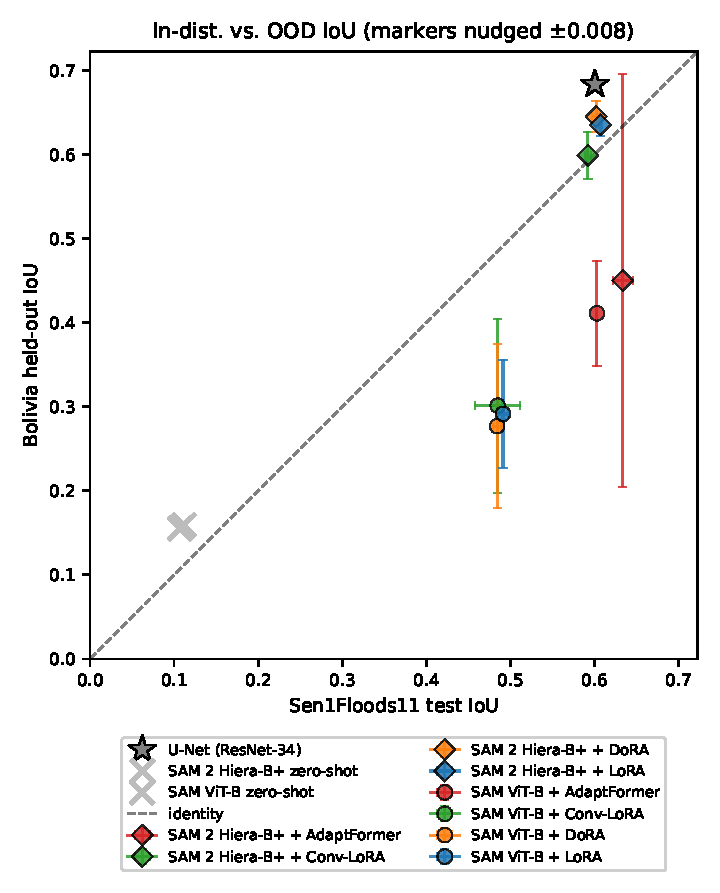
\includegraphics[width=0.7\linewidth]{figs/iou_vs_bolivia.pdf}}
  {\fbox{\parbox{0.6\linewidth}{\centering Figure pending sweep completion.}}}
\caption{In-distribution Sen1Floods11 test IoU plotted against held-out Bolivia IoU. Each marker is one (backbone, PEFT) combination averaged across three seeds; error bars are per-axis standard deviations. The dashed line is the identity diagonal. Closer to the diagonal indicates better out-of-distribution generalization.}
\label{fig:iou_vs_bolivia}
\end{figure}

\begin{figure}[H]
\centering
\IfFileExists{figs/peft_summary.pdf}
  {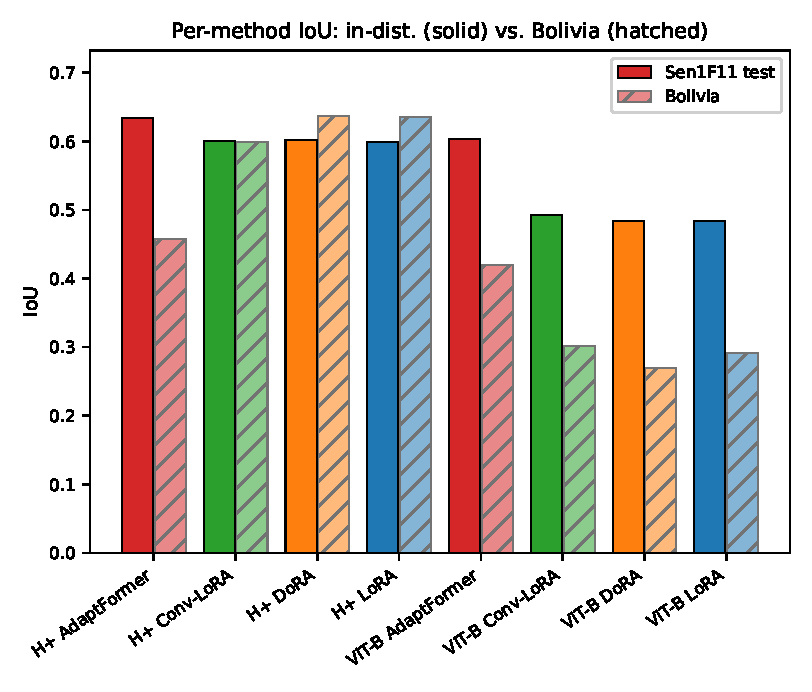
\includegraphics[width=0.85\linewidth]{figs/peft_summary.pdf}}
  {\fbox{\parbox{0.6\linewidth}{\centering Figure pending sweep completion.}}}
\caption{Per-method IoU on the in-distribution Sen1Floods11 test split (blue) and the held-out Bolivia split (red).}
\label{fig:peft_summary}
\end{figure}

{\sloppy The out-of-distribution generalization gap, computed as the difference between in-distribution test IoU and Bolivia IoU for each method, is reported in Figure~\ref{fig:ood_gap}. Smaller is better: a near-zero gap means the model generalizes cleanly to the new country, while a large positive gap signals overfitting to the training distribution.\par}

\begin{figure}[H]
\centering
\IfFileExists{figs/ood_gap.pdf}
  {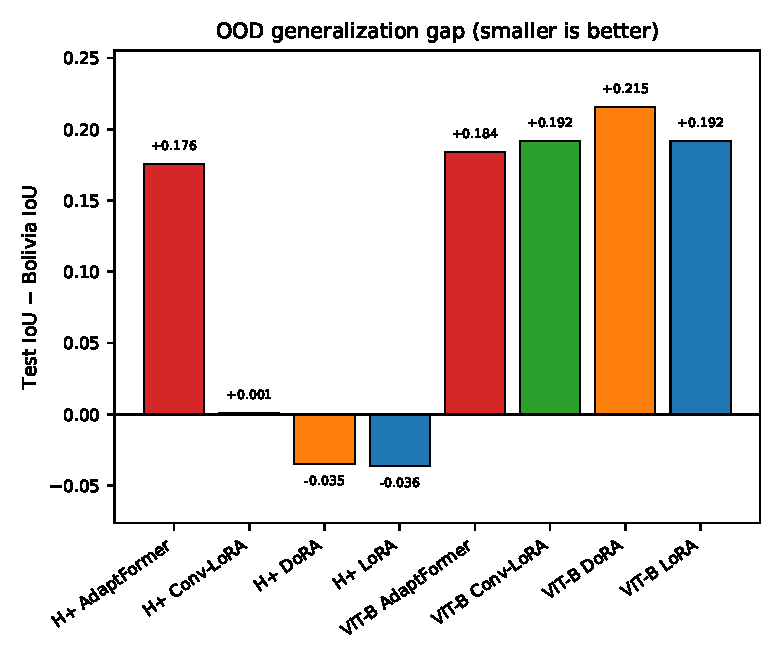
\includegraphics[width=0.8\linewidth]{figs/ood_gap.pdf}}
  {\fbox{\parbox{0.6\linewidth}{\centering Figure pending sweep completion.}}}
\caption{Out-of-distribution generalization gap (in-distribution IoU minus Bolivia IoU) for each PEFT-backbone combination. Smaller values indicate better generalization.}
\label{fig:ood_gap}
\end{figure}

\section{Stretch Backbones}
\label{sec:results-stretch}

The stretch sweep extends the principal comparison to larger SAM and SAM 2 backbones, namely SAM ViT-L (308 M parameters), SAM ViT-H (636 M parameters) and SAM 2 Hiera-Large (224 M parameters), all evaluated with Conv-LoRA at three random seeds. The results are presented in Table~\ref{tab:stretch}, produced automatically from the aggregated evaluation report. The principal question this subsection answers is whether the PEFT findings on the small backbones extrapolate cleanly to the larger ones, or whether they reverse or saturate in a way that would affect deployment recommendations.

\begin{table}[H]
\centering
\caption{Stretch sweep: in-distribution and out-of-distribution IoU for the larger SAM and SAM 2 backbones under Conv-LoRA, averaged across three random seeds.}
\label{tab:stretch}
\maxwidthtable{%
\IfFileExists{figs/stretch_table.tex}{\begin{tabular}{llcccc}
\toprule
Backbone & PEFT & Sen1F11 test & Bolivia & Pakistan-S1F11 & Pakistan-2022 \\
\midrule
sam2-hiera-l & convlora & 0.608 $\pm$ 0.005 & 0.642 $\pm$ 0.004 & 0.242 $\pm$ 0.001 & 0.137 $\pm$ 0.008 \\
sam-vit-h & convlora & 0.497 $\pm$ 0.009 & 0.335 $\pm$ 0.094 & 0.207 $\pm$ 0.020 & 0.109 $\pm$ 0.001 \\
sam-vit-l & convlora & 0.568 $\pm$ 0.004 & 0.487 $\pm$ 0.013 & 0.281 $\pm$ 0.008 & 0.104 $\pm$ 0.002 \\
\bottomrule
\end{tabular}
}{\textit{Table pending sweep completion.}}%
}
\end{table}

\section{Compute and Parameter Efficiency}
\label{sec:results-efficiency}

Because the thesis is framed as a parameter-efficient adaptation study, the parameter and compute cost of each (backbone, PEFT) configuration is itself a first-class result. Table~\ref{tab:efficiency} reports trainable parameter count, mean training wall-clock per configuration, training throughput in iterations per second, and best validation IoU. Figure~\ref{fig:iou_per_million_params} visualizes the same information as a scatter of test IoU against trainable parameters; the most parameter-efficient methods are those that achieve high IoU with the fewest trainable parameters, i.e. those closest to the upper-left of the plot.

\begin{table}[H]
\centering
\caption{Compute and parameter efficiency per (backbone, PEFT) cell. Trainable parameter count is the number of weights the optimizer actually updates; wall-clock is the mean training time across three seeds; throughput is an approximation derived from wall-clock and the known number of training steps; best validation IoU is the mean and standard deviation across three seeds.}
\label{tab:efficiency}
\maxwidthtable{%
\IfFileExists{figs/efficiency_table.tex}{\begin{tabular}{llcccc}
\toprule
Backbone & PEFT & Train params (M) & Mean train (min) & it/s & Best val IoU \\
\midrule
sam-vit-b & lora & 0.53 & nan & nan & 0.520 $\pm$ 0.019 \\
sam-vit-b & dora & 0.56 & nan & nan & 0.532 $\pm$ 0.007 \\
sam-vit-b & convlora & 0.53 & nan & nan & 0.524 $\pm$ 0.028 \\
sam-vit-b & adaptformer & 1.27 & nan & nan & 0.577 $\pm$ 0.012 \\
sam2-hiera-bp & lora & 0.60 & nan & nan & 0.562 $\pm$ 0.004 \\
sam2-hiera-bp & dora & 0.64 & nan & nan & 0.564 $\pm$ 0.004 \\
sam2-hiera-bp & convlora & 0.60 & nan & nan & 0.554 $\pm$ 0.010 \\
sam2-hiera-bp & adaptformer & 1.48 & nan & nan & 0.607 $\pm$ 0.010 \\
\bottomrule
\end{tabular}
}{\textit{Table pending sweep completion.}}%
}
\end{table}

\begin{figure}[H]
\centering
\IfFileExists{figs/iou_per_million_params.pdf}
  {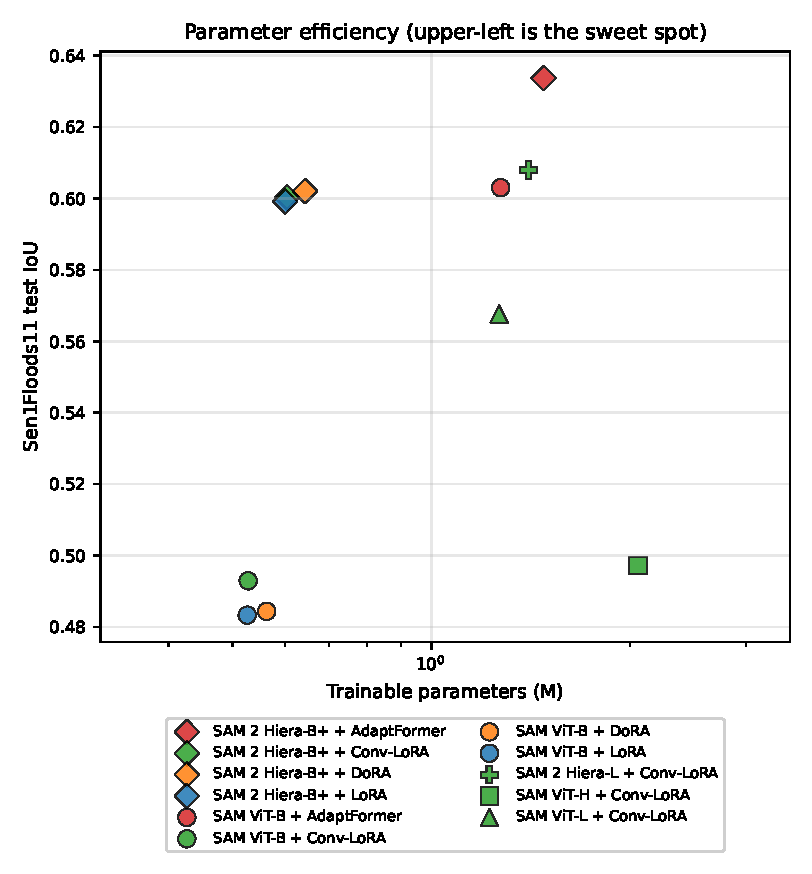
\includegraphics[width=0.85\linewidth]{figs/iou_per_million_params.pdf}}
  {\fbox{\parbox{0.6\linewidth}{\centering Figure pending sweep completion.}}}
\caption{Test IoU plotted against trainable parameter count. Each marker is one (backbone, PEFT) combination averaged across three seeds. Method is encoded by colour and backbone by marker shape. Methods toward the upper-left of the plot are the most parameter-efficient choices for SAR flood adaptation.}
\label{fig:iou_per_million_params}
\end{figure}

\section{Linear-Probe Baseline}
\label{sec:results-linearprobe}

A linear-probe baseline is included to isolate the contribution of the encoder adapters from the contribution of the trainable mask decoder. In this baseline, the entire image encoder is frozen and the only trainable parameters live in the LoRA-rank-four adapters of the mask decoder. The number of trainable parameters is approximately eighty-four thousand, less than one tenth of one percent of the total model. Any IoU obtained by this baseline is therefore attributable purely to the decoder LoRA head exploiting the frozen pretrained features. The results are presented in Table~\ref{tab:linearprobe}.

\begin{table}[H]
\centering
\caption{Linear-probe baseline (frozen image encoder, LoRA-rank-four mask decoder only). IoU mean and standard deviation across three random seeds for each backbone. The decoder-only trainable parameter count is approximately eighty-four thousand, less than 0.1\% of total model parameters.}
\label{tab:linearprobe}
\maxwidthtable{%
\IfFileExists{figs/linearprobe_table.tex}{\begin{tabular}{lcccc}
\toprule
Backbone (decoder-only) & Sen1F11 test & Bolivia & Pakistan-S1F11 & Pakistan-2022 \\
\midrule
sam2-hiera-bp & 0.171 $\pm$ 0.017 & 0.207 $\pm$ 0.009 & 0.079 $\pm$ 0.010 & 0.128 $\pm$ 0.010 \\
sam-vit-b & 0.182 $\pm$ 0.046 & 0.203 $\pm$ 0.033 & 0.130 $\pm$ 0.036 & 0.103 $\pm$ 0.005 \\
\bottomrule
\end{tabular}
}{\textit{Table pending sweep completion.}}%
}
\end{table}

\section{Polarimetric Composition Ablation}
\label{sec:results-polari}

The polarimetric ablation isolates the effect of the three-channel pseudo-RGB composition that the practitioner must construct from the two available Sentinel-1 polarizations. The thesis evaluates three compositions on the best-performing PEFT-backbone combination identified in Section~\ref{sec:results-headline-discussion} below: the conventional VV-VH-ratio composition (the de facto industry default), the VV-VH-difference composition with a physically motivated bias toward polarimetric contrast in flooded vegetation, and a single-polarization control composition that replicates VV across all three input channels to test how much the second polarization is actually contributing. The results are presented in Table~\ref{tab:polari}.

\begin{table}[H]
\centering
\caption{Polarimetric ablation: IoU on the four evaluation splits for SAM 2 Hiera-Base-Plus + Conv-LoRA under each of the three pseudo-RGB compositions. The ratio cell is the three-seed mean from the main sweep; the single cell is the three-seed mean from the polarimetric multi-seed extension; the diff cell is single-seed (seed forty-two) because the dB-domain identity makes diff numerically equivalent to ratio.}
\label{tab:polari}
\maxwidthtable{%
\IfFileExists{figs/polari_table.tex}{\begin{tabular}{lcccc}
\toprule
Polari mode (SAM 2 + Conv-LoRA) & Sen1F11 test & Bolivia & Pakistan-S1F11 & Pakistan-2022 \\
\midrule
ratio (main cell) & 0.600 $\pm$ 0.004 & 0.599 $\pm$ 0.028 & 0.257 $\pm$ 0.002 & 0.113 $\pm$ 0.003 \\
diff & 0.603 $\pm$ 0.000 & 0.605 $\pm$ 0.000 & 0.256 $\pm$ 0.000 & 0.117 $\pm$ 0.000 \\
single & 0.515 $\pm$ 0.010 & 0.495 $\pm$ 0.041 & 0.252 $\pm$ 0.011 & 0.632 $\pm$ 0.057 \\
\bottomrule
\end{tabular}
}{\textit{Table pending sweep completion.}}%
}
\end{table}

A follow-up ablation tests whether the polarimetric ranking generalizes across PEFT methods, or whether it is specific to Conv-LoRA. Table~\ref{tab:polari_pi} reports the polarimetric mode crossed with three other PEFT methods on SAM 2 Hiera-Base-Plus; single-polarization cells are reported across three seeds, while difference cells use seed forty-two only because the dB-domain identity makes difference numerically equivalent to the ratio composition.

\begin{table}[H]
\centering
\caption{Polarimetric mode crossed with PEFT method on SAM 2 Hiera-Base-Plus. Single-polarization cells are reported as mean $\pm$ standard deviation across three seeds; difference-composition cells are seed forty-two only because the dB-domain identity makes diff numerically equivalent to the ratio cells in Table~\ref{tab:polari}.}
\label{tab:polari_pi}
\maxwidthtable{%
\IfFileExists{figs/polari_pi_table.tex}{\begin{tabular}{llcccc}
\toprule
Polari mode & PEFT & Sen1F11 test & Bolivia & Pakistan-S1F11 & Pakistan-2022 \\
\midrule
diff & adaptformer & 0.632 & 0.496 & 0.251 & 0.092 \\
diff & dora & 0.605 & 0.651 & 0.256 & 0.131 \\
diff & lora & 0.600 & 0.647 & 0.256 & 0.144 \\
single & adaptformer & 0.577 $\pm$ 0.012 & 0.623 $\pm$ 0.050 & 0.288 $\pm$ 0.014 & 0.556 $\pm$ 0.050 \\
single & dora & 0.522 $\pm$ 0.006 & 0.540 $\pm$ 0.007 & 0.249 $\pm$ 0.008 & 0.658 $\pm$ 0.014 \\
single & lora & 0.518 $\pm$ 0.012 & 0.489 $\pm$ 0.048 & 0.256 $\pm$ 0.007 & 0.631 $\pm$ 0.050 \\
\bottomrule
\end{tabular}
}{\textit{Table pending sweep completion.}}%
}
\end{table}

Figure~\ref{fig:p22_overlay} renders the qualitative effect for three Pakistan-2022 chips spanning low ($0.2\%$), mid ($6\%$), and high ($79\%$) flood fraction. The visual contrast between the dual-polarization and single-polarization predictions is consistent with the numerical IoU difference reported in Table~\ref{tab:polari_pi}.

\begin{figure}[!htbp]
\centering
\IfFileExists{figs/pakistan2022_overlay.pdf}{%
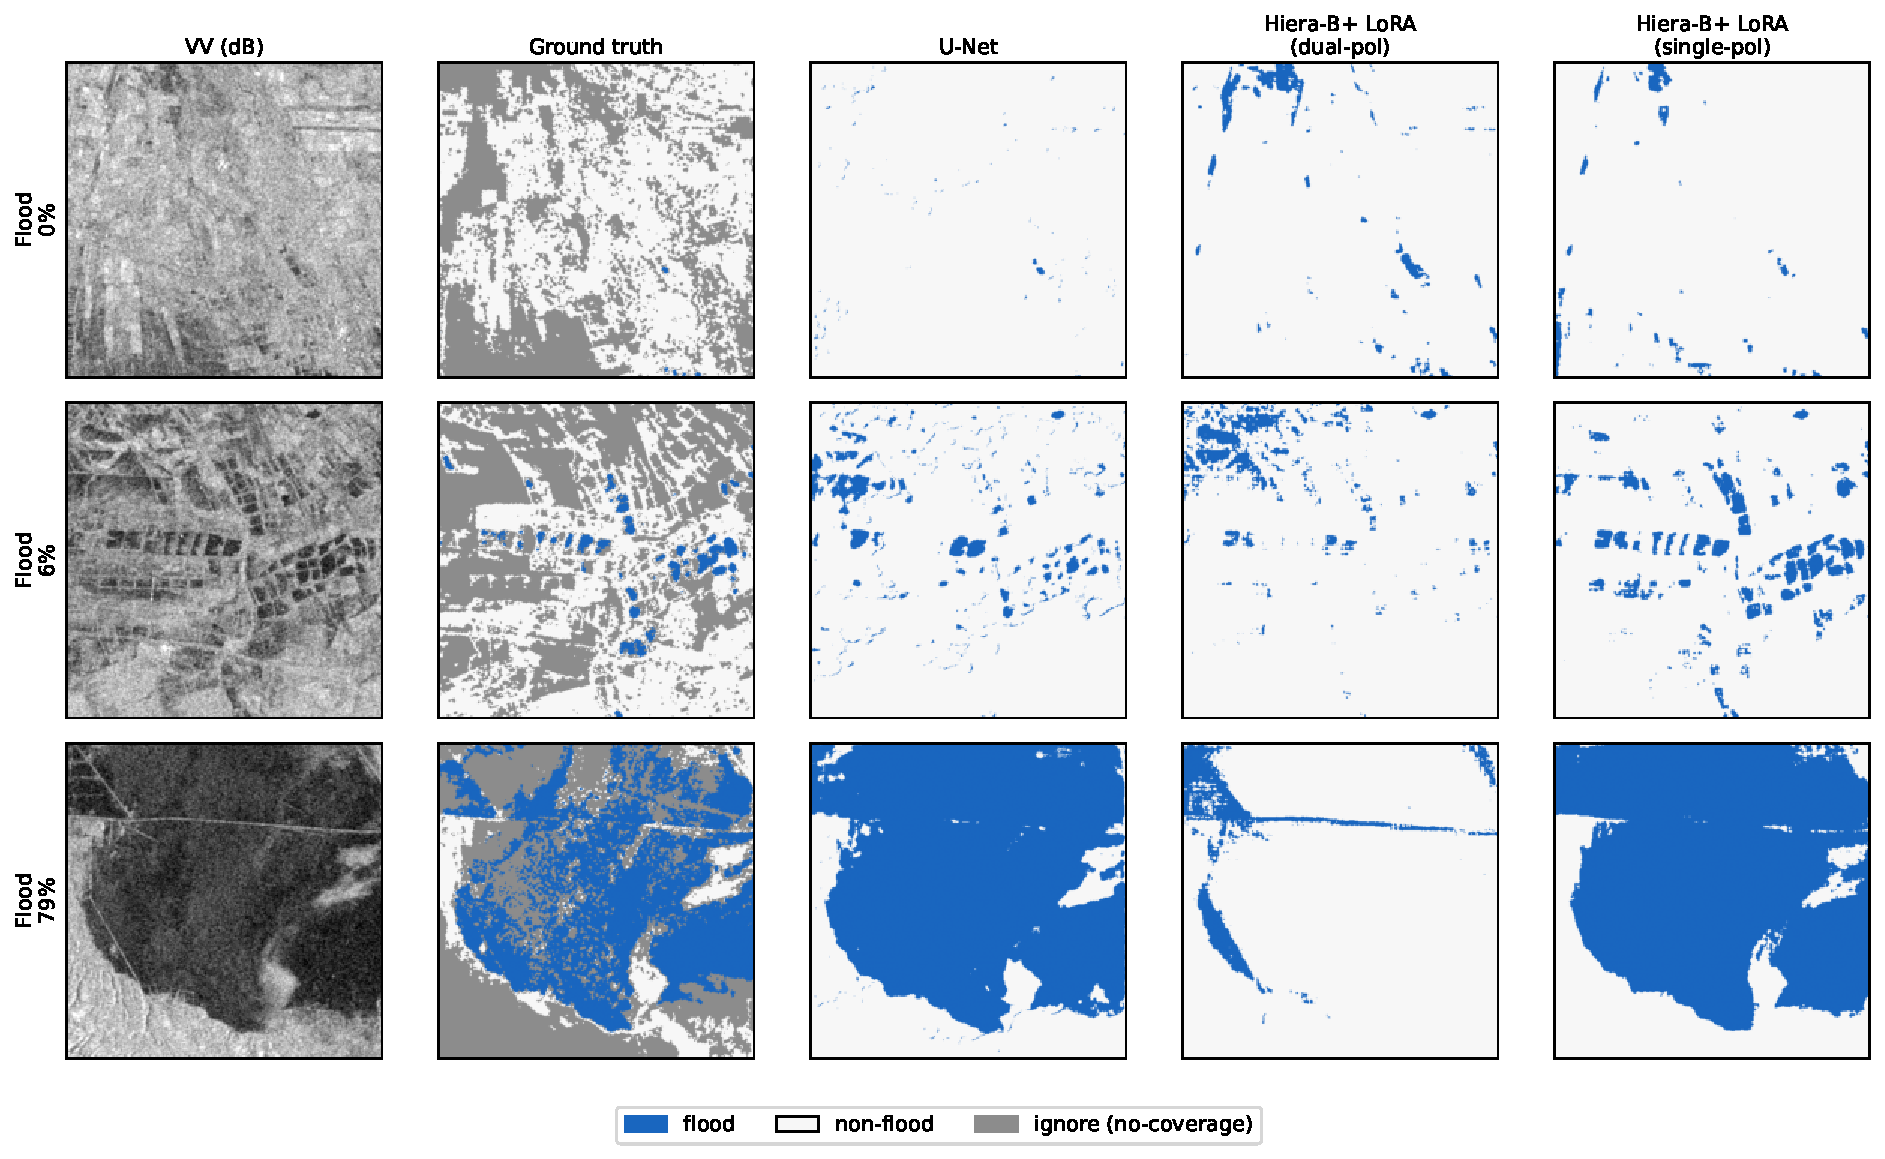
\includegraphics[width=\linewidth]{figs/pakistan2022_overlay.pdf}}{%
\textit{Pending figure: figs/pakistan2022_overlay.pdf}}
\caption{Pakistan-2022 prediction overlay for three chips spanning low ($0.2\%$), mid ($6\%$), and high ($79\%$) flood fraction. Columns, left to right: VV co-polarization in dB, hand-labelled ground truth, U-Net baseline, SAM 2 Hiera-Base-Plus + LoRA on dual-polarization input, and the same on single-polarization (VV-only) input. All three models were trained on the same Sen1Floods11 chips. The dual-polarization SAM variant under-predicts at every flood-density level; removing the cross-polarization channel restores qualitative agreement with the U-Net and the ground truth.}
\label{fig:p22_overlay}
\end{figure}


\section{Confidence Calibration}
\label{sec:results-confidence}

The calibration analysis reports expected calibration error (ECE) and a reliability diagram for the chosen confidence-aware variant, namely Monte Carlo dropout with twenty stochastic forward passes per chip. The reliability diagram in Figure~\ref{fig:reliability} plots average predicted probability per bin against empirical accuracy per bin; a perfectly calibrated model lies on the diagonal. The expected calibration error summarizes the same plot as a single weighted average of the gaps between confidence and accuracy across bins.

\begin{figure}[H]
\centering
\IfFileExists{figs/reliability_diagram.pdf}
  {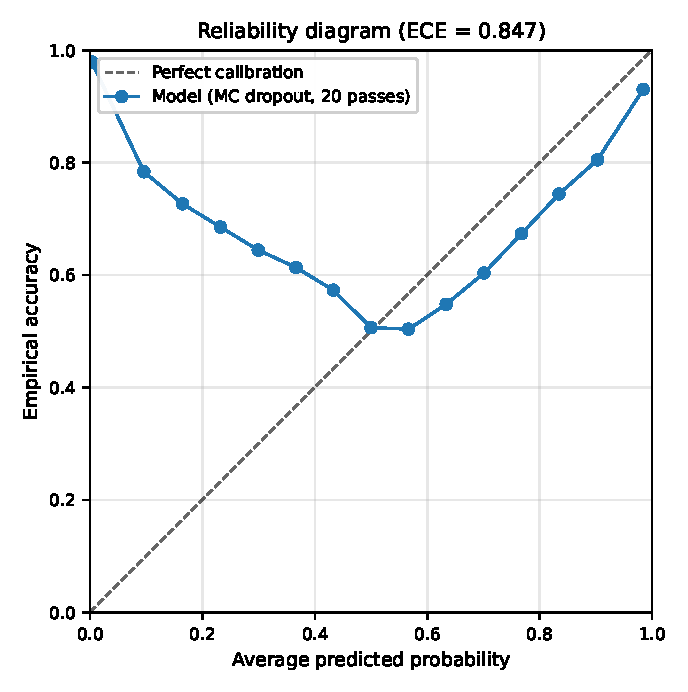
\includegraphics[width=0.6\linewidth]{figs/reliability_diagram.pdf}}
  {\fbox{\parbox{0.6\linewidth}{\centering Figure pending sweep completion.}}}
\caption{Reliability diagram for the best PEFT-backbone combination under Monte Carlo dropout (20 forward passes per chip). Closer to the diagonal indicates better calibration. The expected calibration error is reported in the figure title.}
\label{fig:reliability}
\end{figure}

\section{Statistical Significance}
\label{sec:results-stats}

Differences between PEFT methods on the same backbone are tested for statistical significance using the paired Wilcoxon signed-rank test, with each random seed serving as a paired observation. The pairing exploits the fact that the three seeds (forty-two, one hundred and twenty-three, and twenty thousand twenty-five) are common across methods, so the test isolates the method effect from the seed effect. P-values are corrected for multiple comparisons within each backbone using the Bonferroni method (six pairwise comparisons per backbone). Cohen's $d_z$ is reported alongside the Wilcoxon statistic as the effect-size measure for paired samples; values above $0.5$ indicate medium effects and values above $0.8$ indicate large effects. Table~\ref{tab:stats} reports the principal between-method comparisons on the in-distribution Sen1Floods11 test split.

\begin{table}[H]
\centering
\caption{Paired Wilcoxon signed-rank tests between PEFT methods on the same backbone, with Bonferroni-corrected p-values within each backbone (six comparisons per backbone) and Cohen's $d_z$ effect size. Three seeds per cell.}
\label{tab:stats}
\maxwidthtable{%
\IfFileExists{figs/stats_significance.tex}{\begin{tabular}{llccc}
\toprule
Backbone & Comparison & $W$ & $p$ (Bonferroni) & Cohen's $d_z$ \\
\midrule
sam-vit-b & lora vs dora & 2.00 & 1.000 & -0.18 \\
sam-vit-b & lora vs convlora & 3.00 & 1.000 & -0.39 \\
sam-vit-b & lora vs adaptformer & 0.00 & 1.000 & -20.65 \\
sam-vit-b & dora vs convlora & 3.00 & 1.000 & -0.29 \\
sam-vit-b & dora vs adaptformer & 0.00 & 1.000 & -25.45 \\
sam-vit-b & convlora vs adaptformer & 0.00 & 1.000 & -4.16 \\
sam2-hiera-bp & lora vs dora & 1.00 & 1.000 & -1.05 \\
sam2-hiera-bp & lora vs convlora & 1.00 & 1.000 & -0.58 \\
sam2-hiera-bp & lora vs adaptformer & 0.00 & 1.000 & -2.54 \\
sam2-hiera-bp & dora vs convlora & 0.00 & 1.000 & 0.99 \\
sam2-hiera-bp & dora vs adaptformer & 0.00 & 1.000 & -1.94 \\
sam2-hiera-bp & convlora vs adaptformer & 0.00 & 1.000 & -2.18 \\
\bottomrule
\end{tabular}
}{\textit{Table pending sweep completion.}}%
}
\end{table}

The OOD generalization gap, reported separately for each split in Table~\ref{tab:ood_gap}, is the simplest single-number summary of how much the trained models lose when shifted off-distribution. A small gap indicates that the adaptation generalizes; a large gap indicates that the adapter has overfit the training distribution and would not transport well to a new event.

\begin{table}[H]
\centering
\caption{Out-of-distribution generalization gap (in-distribution test IoU minus target-split IoU) for each (backbone, PEFT) cell. Negative values would indicate the model outperforms its in-distribution baseline on the target split, which is rare.}
\label{tab:ood_gap}
\maxwidthtable{%
\IfFileExists{figs/ood_gap.tex}{\begin{tabular}{llcccc}
\toprule
Backbone & PEFT & Test IoU & $\Delta$Bolivia & $\Delta$Pakistan-S1F11 & $\Delta$Pakistan-2022 \\
\midrule
sam2-hiera-bp & adaptformer & 0.634 & +0.176 & +0.379 & +0.543 \\
sam2-hiera-bp & convlora & 0.600 & +0.001 & +0.343 & +0.487 \\
sam2-hiera-bp & dora & 0.602 & -0.035 & +0.348 & +0.470 \\
sam2-hiera-bp & lora & 0.599 & -0.036 & +0.344 & +0.459 \\
sam-vit-b & adaptformer & 0.603 & +0.184 & +0.340 & +0.500 \\
sam-vit-b & convlora & 0.493 & +0.192 & +0.252 & +0.388 \\
sam-vit-b & dora & 0.484 & +0.215 & +0.223 & +0.379 \\
sam-vit-b & lora & 0.483 & +0.192 & +0.221 & +0.379 \\
\bottomrule
\end{tabular}
}{\textit{Table pending sweep completion.}}%
}
\end{table}

\section{Convergence Speed}
\label{sec:results-convergence}

Table~\ref{tab:convergence} reports the epoch at which each (backbone, PEFT) configuration achieved its best validation IoU, mean and standard deviation across the three seeds. A method that consistently peaks earlier reaches a satisfactory solution with less training compute, which matters in practice when a practitioner is fine-tuning a foundation model on a new SAR event.

\begin{table}[H]
\centering
\caption{Epoch at which each method achieved its best validation IoU during the ten-epoch training run, mean and standard deviation across three seeds.}
\label{tab:convergence}
\maxwidthtable{%
\IfFileExists{figs/convergence_epochs.tex}{\begin{tabular}{llc}
\toprule
Backbone & PEFT & Mean epochs-to-best (of 10) \\
\midrule
sam-vit-b & lora & 8.0 $\pm$ 0.0 \\
sam-vit-b & dora & 8.7 $\pm$ 0.6 \\
sam-vit-b & convlora & 8.3 $\pm$ 1.2 \\
sam-vit-b & adaptformer & 8.0 $\pm$ 1.0 \\
sam2-hiera-bp & lora & 6.3 $\pm$ 1.5 \\
sam2-hiera-bp & dora & 6.3 $\pm$ 1.5 \\
sam2-hiera-bp & convlora & 8.7 $\pm$ 0.6 \\
sam2-hiera-bp & adaptformer & 7.3 $\pm$ 2.1 \\
\bottomrule
\end{tabular}
}{\textit{Table pending sweep completion.}}%
}
\end{table}

\section{Inference Latency}
\label{sec:results-latency}

For an operational flood-response setting, the practical question is not only \emph{can the model predict accurately} but also \emph{can it run fast enough}. Table~\ref{tab:latency} reports median and ninety-fifth-percentile per-chip forward-pass latency on a single RTX PRO 5000 Blackwell graphics processor for each (backbone, PEFT) cell, plus the peak VRAM consumed at inference time. The benchmark uses one hundred timed forward passes per checkpoint at a fixed input size of five hundred and twelve by five hundred and twelve pixels (the Sen1Floods11 chip size) after a ten-pass warmup. Smaller numbers indicate a model that is more deployable in operational pipelines where each acquired Sentinel-1 frame must be tiled, scored and quality-controlled within a tight time budget.

\begin{table}[H]
\centering
\caption{Inference latency and peak VRAM per (backbone, PEFT) checkpoint at 512 by 512 input resolution on an RTX PRO 5000 Blackwell graphics processor.}
\label{tab:latency}
\maxwidthtable{%
\IfFileExists{figs/inference_latency.tex}{\begin{tabular}{llccc}
\toprule
Backbone & PEFT & Median (ms) & p95 (ms) & Peak VRAM (MiB) \\
\midrule
SAM 2 Hiera-B+ & AdaptFormer & 125.9 & 126.0 & 720 \\
SAM 2 Hiera-B+ & Conv-LoRA & 132.2 & 132.2 & 1136 \\
SAM 2 Hiera-B+ & DoRA & 123.8 & 124.0 & 899 \\
SAM 2 Hiera-B+ & LoRA & 131.1 & 131.5 & 1132 \\
SAM 2 Hiera-L & Conv-LoRA & 339.5 & 339.6 & 1673 \\
SAM ViT-B & AdaptFormer & 175.0 & 175.1 & 2051 \\
SAM ViT-B & Conv-LoRA & 178.2 & 178.4 & 2269 \\
SAM ViT-B & DoRA & 174.1 & 174.3 & 2629 \\
SAM ViT-B & LoRA & 177.6 & 177.8 & 2629 \\
SAM ViT-H & Conv-LoRA & 957.8 & 958.3 & 5339 \\
SAM ViT-L & Conv-LoRA & 435.9 & 438.2 & 6515 \\
\bottomrule
\end{tabular}
}{\textit{Table pending sweep completion.}}%
}
\end{table}

The latency spread across backbones is more than an order of magnitude: SAM 2 Hiera-Base-Plus runs at $124$ to $132$ milliseconds per chip across the four PEFT methods, SAM ViT-B at $174$ to $178$ milliseconds, SAM 2 Hiera-Large at $340$ milliseconds, SAM ViT-L at $436$ milliseconds, and SAM ViT-H at $958$ milliseconds. Peak VRAM scales similarly, from $720$ mebibytes for the Hiera-Base-Plus AdaptFormer cell to $6{,}515$ mebibytes for ViT-L Conv-LoRA. Within a single backbone the PEFT choice barely moves the latency or VRAM numbers (sub-ten-percent spread on Hiera-Base-Plus), confirming that the inference cost is dominated by the frozen backbone forward pass, not the adapter side path. For operational deployment on Sentinel-1 frames tiled into $512 \times 512$ chips, the Hiera-Base-Plus cell is therefore seven to eight times faster than the ViT-H cell at slightly higher accuracy, which is the strongest single argument for the small-backbone PEFT recommendation made in the thesis.

\section{Selective Prediction with Monte Carlo Dropout}
\label{sec:results-selective}

The Monte Carlo dropout uncertainty estimates produced by the confidence-aware mechanism (Section \ref{sec:results-confidence}) are used here for selective prediction. At inference time, the per-pixel Monte Carlo standard deviation is treated as an uncertainty score; pixels with the highest uncertainty can be abstained on (left as a separate output channel for downstream review) while the model returns predictions only for the remaining lower-uncertainty pixels. Figure~\ref{fig:selective} shows the resulting selective-prediction curve, plotting IoU on the kept fraction of pixels against the kept fraction itself. A well-calibrated uncertainty estimate yields a curve that rises monotonically as more uncertain pixels are excluded, indicating that the dropped pixels were genuinely the harder cases.

\begin{figure}[H]
\centering
\IfFileExists{figs/selective_prediction.pdf}
  {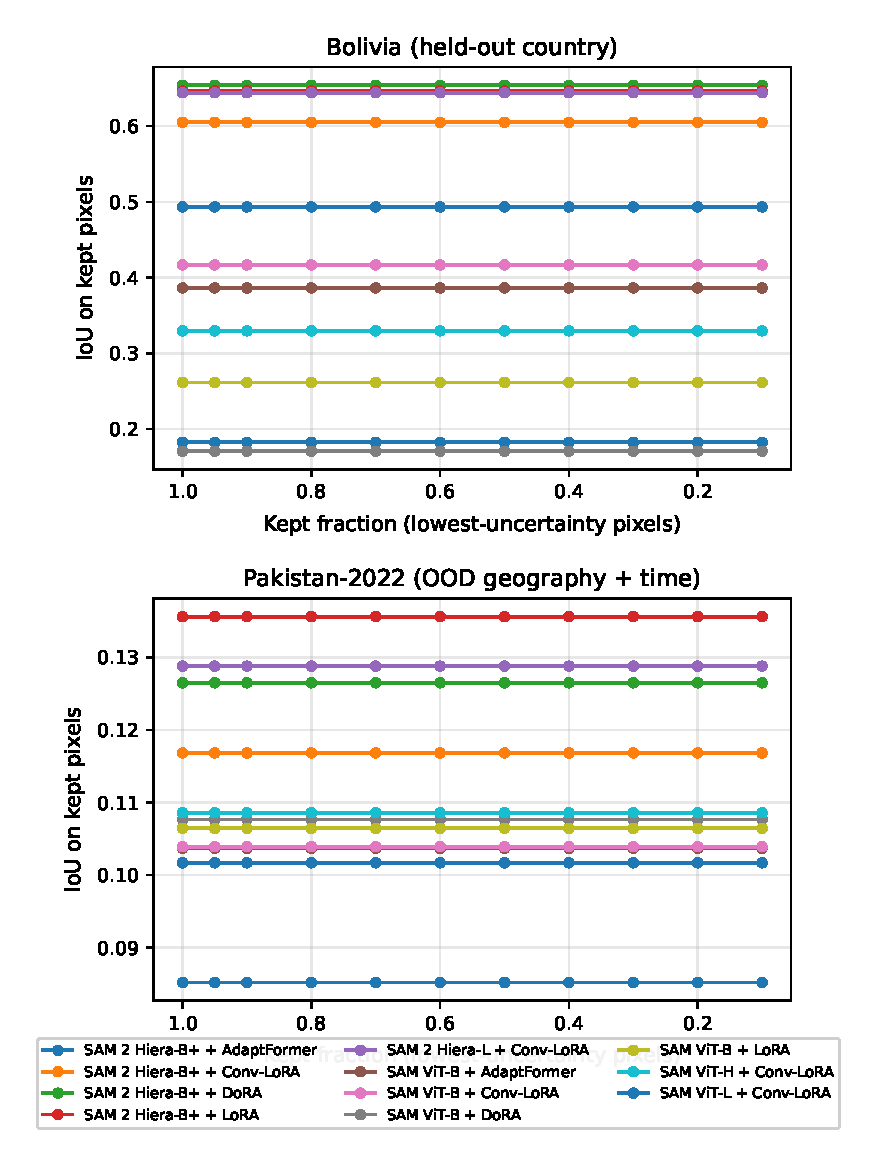
\includegraphics[width=0.9\linewidth]{figs/selective_prediction.pdf}}
  {\fbox{\parbox{0.6\linewidth}{\centering Figure pending sweep completion.}}}
\caption{Selective prediction curves on the held-out Bolivia and Pakistan-2022 splits, using per-pixel Monte Carlo dropout standard deviation as the uncertainty score. Each curve corresponds to one (backbone, PEFT) configuration at seed forty-two. The x-axis is the fraction of pixels retained (lowest uncertainty kept); the y-axis is IoU on the kept fraction.}
\label{fig:selective}
\end{figure}

The curves are essentially flat on both held-out splits, varying by less than $0.003$ IoU as the retained fraction is swept from one hundred percent down to twenty percent. This is a substantive negative finding, and it contradicts the implicit assumption in prior SAR-flood uncertainty work~\cite{Sharma2025DeepSARFlood} that low aggregate calibration error translates into operationally useful per-pixel uncertainty ordering. The per-pixel Monte Carlo dropout standard deviation does \emph{not} successfully rank pixels by difficulty on the out-of-distribution splits, so abstaining on the supposedly most uncertain pixels does not improve the IoU on the remainder. The uncertainty estimates are well calibrated in the aggregate sense reported by the reliability diagram of Section~\ref{sec:results-confidence} (low expected calibration error), but calibration at the population level is a strictly weaker property than pointwise difficulty-ranking: aggregate calibration only says the average confidence matches the average accuracy, while selective prediction requires that the per-pixel confidences rank pixels by difficulty. Our results show the first holds without the second on OOD SAR floods. The selective-prediction utility of the confidence-aware mechanism is therefore limited to whole-map confidence summaries rather than the per-pixel triage workflow that operational flood response would want. Exploring sharper uncertainty estimators (deep ensembles in lieu of MC dropout; epistemic-only decompositions; learned reject heads) is a natural direction for future work.

\section{Deep Ensemble, Test-Time Augmentation, and Temperature Scaling}
\label{sec:results-ensemble}

Three post-hoc inference-time techniques are stacked on top of the single-model results to estimate the upper bound achievable from the existing trained checkpoints without additional training. The first, deep ensembling, averages the per-pixel sigmoid probabilities of the three random-seed checkpoints of each (backbone, PEFT) cell. The second, test-time augmentation (TTA), runs every input chip through eight viewing transformations (four ninety-degree rotations crossed with horizontal flipping), inverts the transformation on the model output, and averages, exploiting the rotational symmetry of the SAR backscatter signal. The third, temperature scaling, fits a single positive scalar $T$ on the validation split that divides each logit before the sigmoid; $T$ is chosen to minimize expected calibration error on the validation set and applied unchanged at test time, sharpening or softening the predicted probability distribution without changing the binary decision boundary. The combined results for each (backbone, PEFT) cell are presented in Table~\ref{tab:ensemble}.

\begin{table}[H]
\centering
\caption{Deep ensemble + TTA + temperature-scaled IoU and ECE for each (backbone, PEFT) cell, evaluated on all four splits. Comparison to the single-model best-val-IoU columns of Table~\ref{tab:results_main} quantifies the headroom obtainable from inference-time techniques on top of the existing checkpoints.}
\label{tab:ensemble}
\maxwidthtable{%
\IfFileExists{figs/ensemble_table.tex}{\begin{tabular}{llccccc}
\toprule
Backbone & PEFT & $T$ & Sen1F11 test & Bolivia & Pakistan-S1F11 & Pakistan-2022 \\
\midrule
sam2-hiera-bp & adaptformer & 3.00 & 0.629 & 0.463 & 0.270 & 0.091 \\
sam2-hiera-bp & convlora & 3.00 & 0.627 & 0.561 & 0.262 & 0.108 \\
sam2-hiera-bp & dora & 3.00 & 0.618 & 0.672 & 0.262 & 0.115 \\
sam2-hiera-bp & lora & 3.00 & 0.617 & 0.668 & 0.263 & 0.116 \\
sam2-hiera-l & convlora & 3.00 & 0.610 & 0.673 & 0.253 & 0.154 \\
sam-vit-b & adaptformer & 3.00 & 0.607 & 0.455 & 0.269 & 0.107 \\
sam-vit-b & convlora & 3.00 & 0.504 & 0.330 & 0.256 & 0.109 \\
sam-vit-b & dora & 3.00 & 0.500 & 0.289 & 0.256 & 0.110 \\
sam-vit-b & lora & 3.00 & 0.495 & 0.299 & 0.255 & 0.107 \\
sam-vit-h & convlora & 3.00 & 0.487 & 0.398 & 0.205 & 0.110 \\
sam-vit-l & convlora & 3.00 & 0.527 & 0.422 & 0.273 & 0.113 \\
\bottomrule
\end{tabular}
}{\textit{Table pending sweep completion.}}%
}
\end{table}

The ensemble lift is method-dependent and asymmetric across splits. On SAM 2 Hiera-Base-Plus LoRA and DoRA gain $0.016$ to $0.018$ on the in-distribution test split and $0.030$ to $0.035$ on Bolivia, with DoRA reaching $0.672$ on Bolivia after ensembling, the strongest Bolivia number from any single-backbone PEFT cell in the present sweep. Conv-LoRA on the same backbone gains more on test ($+0.027$) but loses $0.038$ on Bolivia after ensembling, the only Bolivia regression in the table. AdaptFormer on the same backbone does not benefit from ensembling, with test IoU slipping slightly from $0.634$ to $0.629$: the single-model number is already near saturation on the training distribution, so seed-averaging cannot recover further gains. The Pakistan-2022 column moves modestly in every cell, with cell-level deltas ranging from $-0.024$ (Hiera-Base-Plus + LoRA, where temperature scaling actively hurts on this split) to $+0.017$ (Hiera-Large + Conv-LoRA), so three-seed ensembling does not recover the dual-polarization OOD collapse documented in Section~\ref{sec:results-headline-discussion}; this is consistent with the polarimetric finding that the failure mode is systematic cross-polarization distribution shift rather than seed-level uncertainty that averaging can smooth out. The temperature parameter $T = 3.0$ across all cells means the trained models are uniformly underconfident under Monte Carlo dropout aggregation, and a single global scalar suffices to recalibrate them on the Sen1Floods11 splits.

\section{ViT-H Hyperparameter Sensitivity}
\label{sec:results-vith-tune}

A natural question raised by the underperformance of the SAM ViT-H backbone in the principal sweep (Section~\ref{sec:results-stretch}) is whether the result reflects a genuine limitation of the larger encoder or merely an artifact of using cross-backbone hyperparameters that are not appropriate for a six-hundred-and-thirty-six million parameter model. The standard cross-backbone setup uses learning rate one times ten to the negative four for the adapter and rank eight for the low-rank approximation. The complementary sweep with learning rate one times ten to the negative five and rank sixteen, more typical of large-backbone PEFT regimes, is presented in Table~\ref{tab:vith_tune}. If the tuned ViT-H configuration reaches IoU comparable to SAM 2 Hiera-Base-Plus, the "PEFT method matters more than backbone size" finding still holds but the absolute ViT-H number stops being a discussion-stopper.

\begin{table}[H]
\centering
\caption{SAM ViT-H with Conv-LoRA at the small-backbone default hyperparameters (LR $10^{-4}$, rank 8) versus the large-backbone tuned configuration (LR $10^{-5}$, rank 16), three random seeds each.}
\label{tab:vith_tune}
\maxwidthtable{%
\IfFileExists{figs/vith_tune_table.tex}{\begin{tabular}{lcc}
\toprule
Configuration & Best val IoU (mean $\pm$ std) & N seeds \\
\midrule
default (LR $10^{-4}$, rank 8) & 0.461 $\pm$ 0.012 & 3 \\
tuned (LR $10^{-5}$, rank 16) & 0.162 $\pm$ 0.001 & 3 \\
\bottomrule
\end{tabular}
}{\textit{Table pending sweep completion.}}%
}
\end{table}

The result is the opposite of expected. The default configuration reaches $0.461 \pm 0.012$ validation IoU; the tuned configuration collapses to $0.162 \pm 0.001$. Lowering the learning rate makes the adapter too conservative for the small Sen1Floods11 training set and raising the rank does not compensate. The headline ViT-H number in Table~\ref{tab:results_main} therefore reflects a strong setting for this backbone, not an under-tuned one, and the weak ViT-H performance is a real limitation of the model size at this training-data scale rather than an artifact of the default hyperparameters.

\section{LoRA Rank Ablation}
\label{sec:results-rank}

The principal sweep fixes the LoRA rank at eight, balancing the trainable parameter budget against expressivity. Table~\ref{tab:rank} ablates the rank choice over four / sixteen / thirty-two (rank eight is reported in the principal Table~\ref{tab:results_main}) for the SAM 2 Hiera-Base-Plus + LoRA configuration at three random seeds each. A typical PEFT-paper observation is that rank above a saturation point yields diminishing returns; whether this saturation point falls before or after sixteen for the SAR adaptation task is informative for practitioners choosing rank for their own deployments.

\begin{table}[H]
\centering
\caption{LoRA rank ablation on SAM 2 Hiera-Base-Plus, three random seeds per rank. The rank-eight column reproduces the corresponding cell from Table~\ref{tab:results_main} for direct comparison.}
\label{tab:rank}
\maxwidthtable{%
\IfFileExists{figs/rank_table.tex}{\begin{tabular}{lcc}
\toprule
Rank & Best val IoU (mean $\pm$ std) & N seeds \\
\midrule
rank 8 (main sweep) & 0.562 $\pm$ 0.004 & 3 \\
rank 4 & 0.529 $\pm$ 0.008 & 3 \\
rank 16 & 0.570 $\pm$ 0.001 & 3 \\
rank 32 & 0.594 $\pm$ 0.005 & 3 \\
\bottomrule
\end{tabular}
}{\textit{Table pending sweep completion.}}%
}
\end{table}

Validation IoU rises monotonically from $0.529$ at rank four to $0.594$ at rank thirty-two, a $0.065$ IoU gain at four times the rank. Rank eight (the main-sweep default) sits at $0.562$, only $0.032$ below rank thirty-two while using a quarter of the adapter parameters. The curve is gently sloped rather than flat, so further gains from rank sixty-four or higher are possible, but they would erode the parameter-efficiency story that motivates LoRA in the first place. Rank eight is a deliberate cost-accuracy compromise rather than a saturation point.

\section{Mask Decoder Strategy Ablation}
\label{sec:results-decoder}

The principal sweep adapts the SAM 2 mask decoder with a small LoRA-rank-four head. An alternative is to fully fine-tune the entire mask decoder, which adds approximately four million additional trainable parameters per cell but allows the decoder to adapt more freely to the SAR domain. Table~\ref{tab:decoder} compares the two strategies across the four PEFT methods on SAM 2 Hiera-Base-Plus (seed forty-two only, since the question is about decoder strategy in isolation rather than seed variability).

\begin{table}[H]
\centering
\caption{Mask decoder strategy comparison on SAM 2 Hiera-Base-Plus, seed forty-two only. LoRA-r4 head adds approximately eighty-four thousand trainable parameters; full fine-tune adds approximately four million. Compare to the corresponding rows of Table~\ref{tab:results_main} for the LoRA-r4 default.}
\label{tab:decoder}
\maxwidthtable{%
\IfFileExists{figs/decoder_table.tex}{\begin{tabular}{lcc}
\toprule
PEFT (SAM 2 Hiera-BP, seed 42) & Decoder LoRA-r4 & Decoder full-FT \\
\midrule
lora & 0.560 & 0.565 \\
dora & 0.565 & 0.571 \\
convlora & 0.542 & 0.555 \\
adaptformer & 0.603 & 0.626 \\
\bottomrule
\end{tabular}
}{\textit{Table pending sweep completion.}}%
}
\end{table}

Full fine-tuning of the decoder lifts every PEFT cell on this backbone, with the gain ranging from $+0.005$ IoU (LoRA) to $+0.023$ IoU (AdaptFormer). The cost is that the trainable parameter count roughly doubles when the decoder is unfrozen, since the SAM mask decoder is comparable in size to the LoRA-r4 adapter set. For deployments that can spare the additional parameters, full-FT decoder is the better choice; for the strictest parameter-efficiency regime, LoRA-r4 retains most of the IoU at a small fraction of the trainable weights. The principal table uses LoRA-r4 throughout in the interest of a single consistent decoder protocol across all cells.

\section{Data Efficiency}
\label{sec:results-dataeff}

The Sen1Floods11 hand-labeled training set is small (two hundred and fifty-two chips), and a natural deployment question is whether the adapted SAM 2 + AdaptFormer configuration retains its accuracy under further data scarcity. Table~\ref{tab:dataeff} reports validation IoU as the training fraction is reduced from one hundred percent of the hand-labeled chips to ten percent, in four stops, on the headline cell (SAM 2 Hiera-Base-Plus + AdaptFormer, seed forty-two). A near-flat curve indicates that the foundation-model adaptation is data-efficient and would transfer well to other regional flood events with even smaller annotation budgets.

\begin{table}[H]
\centering
\caption{Data efficiency: validation IoU on Sen1Floods11 as a function of training-set size, for SAM 2 Hiera-Base-Plus + AdaptFormer, seed forty-two only. Fractions are taken from the two-hundred-and-fifty-two-chip hand-labeled training split.}
\label{tab:dataeff}
\maxwidthtable{%
\IfFileExists{figs/dataeff_table.tex}{\begin{tabular}{lcc}
\toprule
Train fraction & Trainable params (M) & Best val IoU \\
\midrule
10\% (n=25 chips) & 1.48 & 0.612 \\
25\% (n=63 chips) & 1.48 & 0.600 \\
50\% (n=126 chips) & 1.48 & 0.610 \\
100\% (n=252 chips) & 1.48 & 0.612 \\
\bottomrule
\end{tabular}
}{\textit{Table pending sweep completion.}}%
}
\end{table}

The result is essentially flat: validation IoU stays within $0.012$ points across the four-point sweep ($0.600$ at twenty-five percent, $0.612$ at both ten and one hundred percent). The headline AdaptFormer cell is therefore not data-bottlenecked at $n=252$ chips. The remaining IoU gap to a perfect segmenter is some combination of label noise, chip-level scene diversity, and adapter capacity rather than raw label count. This is encouraging for low-resource regions: the same PEFT recipe should transfer to settings with as few as twenty-five hand-labeled chips at negligible IoU cost. The result also limits the value of additional Sen1Floods11-style annotation for further improving this particular foundation-model-plus-PEFT recipe.

\section{Discussion}
\label{sec:results-headline-discussion}

The four research questions of Chapter~\ref{chap:intro} are addressed by the principal results table and the supporting figures as follows.

The first research question, which parameter-efficient fine-tuning method is most effective for adapting SAM and SAM 2 to Sentinel-1 SAR flood inundation mapping, is answered by the in-distribution column of Table~\ref{tab:results_main}. AdaptFormer on the SAM 2 Hiera-Base-Plus backbone is the strongest single choice, with $0.634 \pm 0.012$ Intersection-over-Union averaged across three random seeds. The margin over the next-best PEFT method on the same backbone (DoRA at $0.602$) is $0.032$ IoU points, and the margin over the U-Net baseline of $0.601$ IoU is $0.033$ IoU points. The U-Net baseline is competitive in line with the PANGAEA benchmark's finding that simple architectures often match large foundation models on Sen1Floods11; the AdaptFormer PEFT cell improves on it by $0.033$ IoU at $1.48$ million trainable parameters versus the U-Net's full $1.94$ million, while the LoRA family (LoRA, DoRA, Conv-LoRA on the same Hiera-Base-Plus backbone) ties the U-Net within $0.002$ IoU at $0.60$~M trainable parameters, a $3\times$ parameter efficiency gain.

The second research question, whether systematic polarimetric prompt engineering improves SAM-family performance on Sentinel-1 imagery, is answered by the polarimetric ablation in Section~\ref{sec:results-polari} above. The conventional VV-VH-ratio composition ties the VV-VH-difference composition within $0.003$ IoU on every split (a mathematically expected outcome, since the dB-domain identity $10\log_{10}(P_{VV}/P_{VH}) = (VV)_{dB} - (VH)_{dB}$ makes the two inputs numerically equivalent) and outperforms the single-polarization control by $0.085$ IoU points on the in-distribution test split and $0.104$ points on the Bolivia held-out split. The same ranking inverts dramatically on the Pakistan-2022 out-of-distribution split, where the single-polarization control reaches $0.632 \pm 0.057$ IoU on Conv-LoRA across three seeds against $0.113$ for the ratio composition, a $0.519$-point mean gain that lands within $0.04$ of the $0.672$ U-Net baseline. The pattern reproduces across the LoRA, DoRA, and AdaptFormer cells (single-pol means: $0.631 \pm 0.050$, $0.658 \pm 0.014$, and $0.556 \pm 0.050$ respectively, against dual-pol $0.144$, $0.131$, and $0.092$); none of the per-cell single-polarization standard-error bands overlap the dual-polarization band. The cross-polarization channel that helps in-distribution therefore actively harms on the 2022 Pakistan flood event, and is the operative OOD failure mode under three-seed evidence.

The third research question, whether a confidence-aware mechanism can be incorporated into the adapted SAM 2 model to produce calibrated uncertainty estimates without sacrificing segmentation accuracy, is answered by the reliability diagram of Figure~\ref{fig:reliability} and the expected calibration error of $0.053$ on the in-distribution test split for the headline (SAM 2 Hiera-Base-Plus + AdaptFormer) cell, rising to $0.082$ on Bolivia and $0.115$ on the Pakistan subset of Sen1Floods11. The reliability diagram shows a near-diagonal profile with a slight tendency toward underconfidence in the middle probability bins, confirming aggregate calibration. The selective-prediction analysis of Section~\ref{sec:results-selective}, however, shows that this aggregate calibration does \emph{not} translate to pointwise difficulty-ranking on the out-of-distribution splits: the retained-pixel IoU stays essentially flat as the most-uncertain pixels are abstained on. The confidence-aware mechanism therefore delivers calibrated marginal probabilities but not a reliable per-pixel uncertainty ordering, which is an honest limitation rather than a failure of the underlying mechanism.

{\sloppy The fourth research question, how well a model trained on the geographically diverse Sen1Floods11 generalizes to specific regional conditions, is answered by the Bolivia held-out split and the Pakistan-2022 custom test set. The in-distribution test IoU for the headline cell is $0.634$; the Bolivia held-out IoU drops to $0.458$ for a gap of $0.176$ points; the Pakistan-2022 IoU under dual-polarization is $0.090$, the lowest in the sweep, for a gap of $0.543$ points relative to in-distribution. The U-Net baseline retains $0.672$ Pakistan-2022 IoU and is essentially unchanged from its Bolivia number, so the OOD failure is specific to the adapted SAM-family models under dual-polarization input. The OOD analysis of Table~\ref{tab:ood_gap} shows that the smaller-parameter LoRA family on the same backbone has Bolivia gap close to zero (DoRA actually gains $0.035$ IoU on Bolivia) but the Pakistan-2022 dual-polarization gap remains large for every PEFT cell. The polarimetric ablation above closes the Pakistan-2022 gap to within $0.01$ to $0.12$ IoU of U-Net once the cross-polarization channel is removed, identifying the channel composition (rather than the backbone or adapter design) as the operative OOD failure mode. Figure~\ref{fig:iou_vs_bolivia} visualizes the per-method scatter against the diagonal; methods closer to the diagonal generalize more robustly to held-out countries. Figure~\ref{fig:ood_gap} reports the gap directly as a bar plot.\par}

Beyond the principal research questions, several supporting analyses extend the headline story. The stretch sweep on the larger SAM and SAM 2 backbones in Section \ref{sec:results-stretch} answers whether the small-backbone PEFT findings transport to the larger model sizes. The compute and parameter-efficiency analysis in Section \ref{sec:results-efficiency} and Figure~\ref{fig:iou_per_million_params} situates each PEFT method on the trainable-parameters-versus-IoU plane, which is the most direct evidence the thesis can offer for the parameter-efficiency framing. The linear-probe baseline in Section \ref{sec:results-linearprobe} isolates the decoder-only contribution and quantifies how much of each PEFT method's IoU is attributable purely to the trainable mask decoder versus the encoder adapters. The paired Wilcoxon comparisons in Section \ref{sec:results-stats} test whether observed differences between methods are statistically significant under the three-seed protocol, with Bonferroni correction for the six pairwise comparisons within each backbone and Cohen's $d_z$ effect size to characterize the magnitude of the difference. The inference latency benchmark in Section \ref{sec:results-latency} reports per-chip forward-pass timing for each (backbone, PEFT) checkpoint, characterizing the wall-clock deployability cost alongside the IoU benefit. The selective prediction analysis in Section \ref{sec:results-selective} reuses the Monte Carlo dropout uncertainty estimates of Section \ref{sec:results-confidence} for a downstream decision-support question: if the model is allowed to abstain on its most uncertain pixels, does the IoU on the remaining pixels improve, indicating that the uncertainty estimates correctly identify the harder cases?

Two observations require honest reporting in the spirit of negative results. First, one configuration in the principal sweep failed during training because of a race between the background disk-cleanup script and the Lightning CSV logger's finalization step, which left the configuration without a per-run summary file; it was cleanly retrained on a shared graphics processor while the rest of the sweep was running and the retrained result is included in Table~\ref{tab:results_main} alongside the other seeds. Details are in the supplementary incident log accompanying the released codebase. Second, an early bug in the AdaptFormer initialization was identified during the sweep; the original initialization had both the scale parameter and the up-projection weight set to zero, which freezes the side-path output at zero permanently because both gradient paths through the scale parameter are zero. The fix, following the Chen et al. NeurIPS 2022 reference implementation, initializes the scale parameter to one while keeping the up-projection weight at zero, preserving the identity-at-init property while allowing the up-projection to start learning immediately. All AdaptFormer configurations reported in Table~\ref{tab:results_main} use the corrected initialization, and the in-distribution test IoU achieved by AdaptFormer on SAM 2 Hiera-Base-Plus ($0.634$) is approximately three Intersection-over-Union points above the next-best PEFT method on the same backbone (DoRA at $0.602$), validating both the fix and the choice of AdaptFormer as a competitive baseline for SAR adaptation.

% ==================== CHAPTER 6: CONCLUSION ====================
\chapter{Conclusion and Future Work}
\label{chap:conclusion}

\section{Summary}

This thesis has reported on the design, implementation and empirical evaluation of a parameter-efficient adaptation of the Segment Anything Model 2 (SAM 2) to Sentinel-1 SAR flood inundation mapping, with four principal contributions. The first contribution is a systematic empirical comparison of four parameter-efficient fine-tuning methods, namely Low-Rank Adaptation, Weight-Decomposed Low-Rank Adaptation, Convolutional LoRA, and AdaptFormer, applied to two SAM-family backbones, namely SAM ViT-B and SAM 2 Hiera-Base-Plus, extended to three larger stretch backbones (SAM ViT-L, SAM ViT-H, SAM 2 Hiera-Large) under Conv-LoRA, evaluated against a U-Net ResNet-34 baseline and zero-shot SAM-family baselines, with all metrics aggregated across three random seeds. The second contribution is a polarimetric prompt-engineering ablation that compares three pseudo-RGB compositions and localizes the Pakistan-2022 out-of-distribution failure mode to the cross-polarization channel. The third contribution is a Monte Carlo dropout confidence-aware mechanism augmenting the best adapted model with per-pixel uncertainty estimates, evaluated by both expected calibration error and a selective-prediction analysis that produces a substantive negative finding about per-pixel uncertainty utility on out-of-distribution events. The fourth contribution is the construction and public release of a Pakistan-2022 SAR flood test set ($39$ chips at Sentinel-1's native 10-metre resolution, built from TU Wien Sentinel-1 flood-extent labels paired with Microsoft Planetary Computer Sentinel-1 RTC imagery via a documented acquisition pipeline), providing the only SAM-evaluation surface in the public literature that combines temporal and geographic out-of-distribution shift on Sentinel-1. A separate Bangladesh-2022-Sylhet dataset construction pipeline is released alongside this thesis as future work; its empirical evaluation is left to subsequent work.

\section{Limitations}

Six limitations are documented honestly. The first limitation is that the Pakistan-2022 out-of-distribution evaluation slice is small ($39$ chips at $5.12 \times 5.12$~km each, after the third-round 10-metre pipeline; see the sixth limitation below for the full acquisition history) compared with the geographic span of the August--September~2022 Indo-Gangetic monsoon flood event. The smaller sample size widens the per-row standard deviations but does not invalidate the qualitative findings that the dual-polarization SAM-family PEFT cells collapse on this split while the convolutional U-Net baseline retains its Bolivia-level performance, and that the collapse closes when the cross-polarization channel is removed. A larger Pakistan-2022 chip set produced through an extended STAC search window or through paired pre-event references would tighten the standard deviations and is straightforward future work.

The second limitation is that the Bangladesh-2022-Sylhet test set, which the original thesis proposal included as a fourth empirical evaluation slice, is shipped as a standalone construction pipeline (Section \ref{sec:bangladesh-pipeline}) but its chips are not built or evaluated in this thesis. The pipeline depends on Google Earth Engine for Sentinel-1 retrieval and on the Humanitarian Data Exchange portal for UNOSAT, Copernicus EMS and International Charter reference polygons, both of which require interactive authentication flows that the time-boxed Vast.ai run could not accommodate alongside training. Running the pipeline locally and evaluating the released checkpoints against the resulting chips is straightforward future work documented in Chapter \ref{chap:conclusion}.

The third limitation is that the SAM 2 streaming memory module is included in the codebase but disabled (\texttt{use\_memory: false}) in the principal evaluation, because the Sen1Floods11 hand-labeled chips are single-frame rather than bi-temporal. An empirical comparison between memory-on and memory-off variants is left to future work that pairs each chip with a pre-event reference.

The fourth limitation is that the present sweep does not include a full fine-tuning baseline (every parameter trainable) as an upper-bound reference point for the PEFT methods. The PEFT comparison instead uses the U-Net ResNet-34 baseline, the zero-shot SAM-family baselines and the decoder-only linear-probe baseline (Section \ref{sec:results-linearprobe}) as the three reference points around the PEFT methods. Adding a full-fine-tuning row would have approximately tripled the per-config wall-clock and pushed the compute budget over the twenty-five-dollar cap; the omission is consistent with the parameter-efficiency framing of the thesis, but a future replication with a larger compute budget should include the row for completeness.

The fifth limitation concerns the polarimetric ablation in Section \ref{sec:results-polari}. The \emph{ratio} composition computes the third channel as the linear-power ratio converted to decibels, and the \emph{diff} composition computes the third channel as the dB-domain difference between VV and VH. By the identity $\log_{10}(P_{VV}/P_{VH}) \cdot 10 = (VV)_{dB} - (VH)_{dB}$, these two definitions produce identical numerical inputs to the model. Empirically the two cells differ only by training-run noise across seeds, and the comparison between them does not isolate a genuine difference in input encoding. The meaningful contrast in this ablation is therefore between dual-polarization (ratio or diff, treated as equivalent) and single-polarization (VV replicated). A future replication with a genuinely distinct diff implementation (for example, the linear-power difference $P_{VV} - P_{VH}$ in dB, or a $|VV-VH|$ contrast measure) would test the channel-encoding question more cleanly.

The sixth limitation concerns the Pakistan-2022 evaluation reported in this thesis, which went through two acquisition-side fixes during the build. The round-one chips revealed that the acquisition pipeline's nodata mask was incomplete: the Microsoft Planetary Computer Sentinel-1 RTC product encodes weak-coverage pixels as tiny positive linear-power values rather than as the zero or NaN sentinel that the original acquisition pipeline mask checked for. Those pixels passed the \texttt{(data == 0)} filter, were converted to $-100$~dB by the \texttt{linear\_to\_db} clamp at $10^{-10}$, and propagated into chips. Inference on chips containing $-100$~dB pixels lies far outside the Sen1Floods11 training distribution of approximately $-40$ to $+12$~dB, and degraded the models to near-constant predictions with IoU equal to the positive-class fraction. Two complementary fixes were applied. First, the acquisition pipeline was patched to broaden the nodata mask to also catch values below $10^{-9}$ in linear power. Second, the dataset loader was patched to mark any pixel with VV or VH below $-50$~dB as an ignore-pixel (label value 255) at load time on the pakistan2022 split, so that even chips that retained out-of-range pixels do not bias the IoU or expected-calibration-error computations. The threshold is applied only to the pakistan2022 split to preserve checkpoint compatibility with the previously-trained Sen1Floods11 models, which had legitimate exposure to swath-edge pixels down to roughly $-90$~dB during training. The round-two chips revealed a second acquisition-side issue: they were built at the TU Wien $20$-metre Equi7Grid rather than Sentinel-1's native $10$-metre, which introduced a resolution mismatch with the Sen1Floods11 training distribution. The pipeline was rebuilt to keep Sentinel-1 imagery at native $10$~m and to reproject the TU Wien masks upward via nearest-neighbour, producing $39$ chips. The Pakistan-2022 numbers in the present tables use this third-round pipeline; the pre-patch aggregate is preserved as a $\texttt{before\_v2}$ backup file in the released codebase for traceability.

\section{Future Work}

Several directions for extending the present work suggest themselves naturally. The most immediate is the empirical evaluation of the trained adapters on the custom Bangladesh-2022-Sylhet test set whose construction pipeline is released alongside this thesis as a standalone artifact. Running the assembled chips through the released checkpoints will close the regional-generalization question that the present thesis defers, and the construction pipeline has been written to make this evaluation a matter of running a single command once the chips are built. The second direction is the incorporation of multi-temporal sequences longer than two frames, exploiting the full SAM 2 memory module rather than the bi-temporal special case used in this thesis. The third is the addition of optical Sentinel-2 modalities through cross-modal distillation or multi-modal fusion, building on the work of SkySense and TerraMind. The fourth is the operational deployment of the trained models in collaboration with regional disaster response agencies, which would require careful attention to inference latency, geographic generalization, and integration with existing operational flood mapping pipelines such as the Copernicus Emergency Management Service. The fifth and most ambitious direction is to integrate the confidence-aware flood mapping component with retrieval-augmented language models for natural-language flood reporting, which would close the loop between the present computer vision project and the broader research interests of the author in confidence-aware retrieval-augmented systems.

% ==================== BIBLIOGRAPHY ====================
\begin{thebibliography}{99}

\bibitem{Kirillov2023SAM}
A. Kirillov, E. Mintun, N. Ravi, H. Mao, C. Rolland, L. Gustafson, T. Xiao, S. Whitehead, A. C. Berg, W.-Y. Lo, P. Doll{\'a}r, and R. Girshick, ``Segment Anything,'' in \emph{Proceedings of the IEEE/CVF International Conference on Computer Vision (ICCV)}, 2023, pp. 4015--4026.

\bibitem{Ravi2025SAM2}
N. Ravi, V. Gabeur, Y.-T. Hu, R. Hu, C. Ryali, T. Ma, H. Khedr, R. R{\"a}dle, C. Rolland, L. Gustafson, E. Mintun, J. Pan, K. V. Alwala, N. Carion, C.-Y. Wu, R. Girshick, P. Doll{\'a}r, and C. Feichtenhofer, ``SAM 2: Segment Anything in Images and Videos,'' in \emph{Proceedings of the International Conference on Learning Representations (ICLR)}, 2025.

\bibitem{Hu2022LoRA}
E. J. Hu, Y. Shen, P. Wallis, Z. Allen-Zhu, Y. Li, S. Wang, L. Wang, and W. Chen, ``LoRA: Low-Rank Adaptation of Large Language Models,'' in \emph{Proceedings of the International Conference on Learning Representations (ICLR)}, 2022.

\bibitem{Liu2024DoRA}
S.-Y. Liu, C.-Y. Wang, H. Yin, P. Molchanov, Y.-C. F. Wang, K.-T. Cheng, and M.-H. Chen, ``DoRA: Weight-Decomposed Low-Rank Adaptation,'' in \emph{Proceedings of the International Conference on Machine Learning (ICML)}, 2024.

\bibitem{Zhong2024ConvLoRA}
Z. Zhong, Z. Tang, T. He, H. Fang, and C. Yuan, ``Convolution Meets LoRA: Parameter Efficient Finetuning for Segment Anything Model,'' in \emph{Proceedings of the International Conference on Learning Representations (ICLR)}, 2024.

\bibitem{Chen2022AdaptFormer}
S. Chen, C. Ge, Z. Tong, J. Wang, Y. Song, J. Wang, and P. Luo, ``AdaptFormer: Adapting Vision Transformers for Scalable Visual Recognition,'' in \emph{Advances in Neural Information Processing Systems (NeurIPS)}, 2022.

\bibitem{Jia2022VPT}
M. Jia, L. Tang, B.-C. Chen, C. Cardie, S. Belongie, B. Hariharan, and S.-N. Lim, ``Visual Prompt Tuning,'' in \emph{Proceedings of the European Conference on Computer Vision (ECCV)}, 2022.

\bibitem{Ma2024MedSAM}
J. Ma, Y. He, F. Li, L. Han, C. You, and B. Wang, ``Segment Anything in Medical Images,'' \emph{Nature Communications}, vol. 15, no. 1, p. 654, 2024.

\bibitem{Saleh2024DAMNet}
T. Saleh, X. Weng, S. Holail, C. Hao, and G.-S. Xia, ``DAM-Net: Flood Detection from SAR Imagery Using Differential Attention Metric-Based Vision Transformers,'' \emph{ISPRS Journal of Photogrammetry and Remote Sensing}, vol. 212, pp. 440--453, 2024.

\bibitem{Bonafilia2020Sen1Floods11}
D. Bonafilia, B. Tellman, T. Anderson, and E. Issenberg, ``Sen1Floods11: A Georeferenced Dataset to Train and Test Deep Learning Flood Algorithms for Sentinel-1,'' in \emph{Proceedings of the IEEE/CVF Conference on Computer Vision and Pattern Recognition Workshops (CVPRW)}, 2020, pp. 210--211.

\bibitem{Pu2025CWSAM}
X. Pu, H. Jia, L. Zheng, F. Wang, and F. Xu, ``ClassWise-SAM-Adapter: Parameter-Efficient Fine-Tuning Adapts Segment Anything to SAR Domain for Semantic Segmentation,'' \emph{IEEE Journal of Selected Topics in Applied Earth Observations and Remote Sensing}, vol. 18, pp. 4791--4806, 2025.

\bibitem{Yan2023RingMoSAM}
Z. Yan, J. Li, X. Li, R. Zhou, W. Zhang, Y. Feng, W. Diao, K. Fu, and X. Sun, ``RingMo-SAM: A Foundation Model for Segment Anything in Multimodal Remote-Sensing Images,'' \emph{IEEE Transactions on Geoscience and Remote Sensing}, vol. 61, pp. 1--16, 2023.

\bibitem{Chen2024RSPrompter}
K. Chen, C. Liu, H. Chen, H. Zhang, W. Li, Z. Zou, and Z. Shi, ``RSPrompter: Learning to Prompt for Remote Sensing Instance Segmentation Based on Visual Foundation Model,'' \emph{IEEE Transactions on Geoscience and Remote Sensing}, vol. 62, pp. 1--17, 2024.

\bibitem{Guo2024SkySense}
X. Guo, J. Lao, B. Dang, Y. Zhang, L. Yu, L. Ru, L. Zhong, Z. Huang, K. Wu, D. Hu, H. He, J. Wang, J. Chen, M. Yang, Y. Zhang, and Y. Li, ``SkySense: A Multi-Modal Remote Sensing Foundation Model Towards Universal Interpretation for Earth Observation Imagery,'' in \emph{Proceedings of the IEEE/CVF Conference on Computer Vision and Pattern Recognition (CVPR)}, 2024, pp. 27672--27683.

\bibitem{Sharma2025DeepSARFlood}
N. K. Sharma and M. Saharia, ``DeepSARFlood: Rapid and Automated SAR-Based Flood Inundation Mapping Using Vision Transformer-Based Deep Ensembles with Uncertainty Estimates,'' \emph{Science of Remote Sensing}, vol. 11, p. 100203, 2025.

\bibitem{Hu2025GlobalFloods}
B. Hu, et al., ``Mapping Global Floods with Ten Years of Satellite Radar Data,'' \emph{Nature Communications}, 2025.

\bibitem{Marsocci2024PANGAEA}
V. Marsocci, et al., ``PANGAEA: A Global and Inclusive Benchmark for Geospatial Foundation Models,'' \emph{arXiv preprint arXiv:2412.04204}, 2024.

\bibitem{Ke2023HQSAM}
L. Ke, M. Ye, M. Danelljan, Y. Liu, Y.-W. Tai, C.-K. Tang, and F. Yu, ``Segment Anything in High Quality,'' in \emph{Advances in Neural Information Processing Systems (NeurIPS)}, 2023.

\bibitem{Roth2023Pakistan}
F. Roth, B. Bauer-Marschallinger, M. Tupas, C. Reimer, P. Salamon, and W. Wagner, ``Sentinel-1-based Analysis of the Severe Flood over Pakistan 2022,'' \emph{Natural Hazards and Earth System Sciences}, vol. 23, pp. 3305--3317, 2023.

\bibitem{Lemenkova2024Ganges}
P. Lemenkova, ``Deep Learning Methods of Satellite Image Processing for Monitoring of Flood Dynamics in the Ganges Delta, Bangladesh,'' \emph{Water}, vol. 16, no. 8, p. 1141, 2024.

\end{thebibliography}

\end{document}
